\documentclass[11pt]{article}
\usepackage{fullpage}
\usepackage{verbatim}
\usepackage{moreverb}
\usepackage{amsmath}
\let\verbatiminput=\verbatimtabinput
\def\verbatimtabsize{4\relax}
\usepackage{tikz}
\usetikzlibrary{arrows,automata, positioning}
\usepackage{array}
\usepackage{booktabs}
\usepackage{minted}
\usepackage{parskip}
\usepackage{float}
\usepackage{pbox}
\usepackage{makecell}
\graphicspath{{images/}}

\usepackage{color}
\definecolor{rltred}{rgb}{0.75,0,0}
\definecolor{rltgreen}{rgb}{0,0.5,0}
\definecolor{rltblue}{rgb}{0,0,0.75}

\usepackage[%pdftex,
    colorlinks=true,
    urlcolor=rltblue,               % \href{...}{...}
    anchorcolor=rltbrightblue,
    filecolor=rltgreen,             % \href*{...}
    linkcolor=rltred,               % \ref{...} and \pageref{...}
    menucolor=webdarkblue,
    citecolor=webbrightgreen,
    pagebackref,
    pdfpagemode=None,
    bookmarksopen=true]{hyperref}
\usepackage{graphicx}
\usepackage{hyperref}

\newcommand{\instbit}[1]{\mbox{\scriptsize #1}}
\newcommand{\instbitrange}[2]{~\instbit{#1} \hfill \instbit{#2}~}

\newcommand{\currentSemester}{Spring 2017}
\newcommand{\projectSpecVersion}{2.0}

\newcommand{\dueDateTime}{5:00 PM}

\newcommand{\labFiveDueDate}{Wednesday, March 8}
\newcommand{\labSixDueDate}{Wednesday, March 15}

\newcommand{\blockDiagramTaskName}{Checkpoint 0.5}
\newcommand{\blockDiagramDueDate}{Wednesday, March 15}
\newcommand{\blockDiagramTimeAlloted}{1 week}

\newcommand{\baseCPUTaskName}{Checkpoint 1}
\newcommand{\baseCPUDueDate}{Wednesday, April 12}
\newcommand{\baseCPUTimeAlloted}{3 weeks}

\newcommand{\audioTaskName}{Checkpoint 2}
\newcommand{\audioDueDate}{Friday, April 14}
\newcommand{\audioTimeAlloted}{1 week}

\newcommand{\ethernetTaskName}{Checkpoint 3}
\newcommand{\ethernetDueDate}{Wednesday, April 26}
\newcommand{\ethernetTimeAlloted}{2 weeks}

\newcommand{\finalCheckoffDueDate}{Friday, May 5}

\newcommand{\skeletonRepoName}{sp17_project_skeleton}
\newcommand{\semesterName}{sp17}

\begin{document}
\begin{center}
{\bf
University of California at Berkeley \\
College of Engineering \\
Department of Electrical Engineering and Computer Science \\
}
\end{center}

\begin{center}
EECS151/251A - LB, \currentSemester
\end{center}

\begin{center}
\LARGE
{\bf Project Specification: RISCV151 }  \\
Version \projectSpecVersion
\end{center}

\tableofcontents

\newpage

\section{Introduction}

The primary goal of this project is to familiarize EECS151/251A students with the methods and tools of digital design.  In teams of 2, you will design and implement a complete 3-stage pipelined version of a RISC-V CPU. In addition to this, you will create a audio (AC97) controller that can stream audio samples to the headphone jack on the FPGA board. A functional implementation will be your primary goal.  To better expose you to real design decisions and tradeoffs, however, we are requiring that you optimize your design for cost (FPGA resource utilization) and performance (maximizing the Iron Law).

You will use Verilog to implement this system, targeting the Xilinx XUPv5 platform (based around the Virtex 5 LX110T FPGA on the ML505 evaluation board). The project will give you experience designing with RTL descriptions, resolving hazards in a simple pipeline, building interfaces, and teach you how to approach system-level optimization.

In tackling these challenges, your first step will be to map our high level specification to a design which can be translated into a hardware implementation.  After that, you will produce and debug that implementation. These first steps can potentially take significant time if you have not thought out your design prior to trying implementation.  After you have built a working implementation, the next step will be optimizing it for area (cost, resource use) on the target FPGA.  You will be expected to produce a relatively minimal circuit, implementing the required functionality, given a clock fixed at a certain frequency.  At the end of this second phase (optimization, post implementation), you should have a greater understanding for the development process of digital hardware.

As in previous semesters, your EECS151/251A project is probably the largest project you have faced so far here at Berkeley. Good time management and good design organization is critical to your success.

\subsection{Philosophy}
\label{philosophy}

This document is meant to describe a high-level specification for the project and its associated support hardware. You can also use it to help lay out a plan for completing the project. As with any design you will encounter in the professional world, we are merely providing a framework within which your project must fit.

You should consider the GSIs a source of direction and clarification, but it is up to you to produce a fully functional design targeting the XUPv5 boards. We will attempt to help, when possible, but ultimately the burden of designing and debugging your solution lies on you.

There is the opportunity to extend our framework with additional functionality for extra credit. This is described in Section \ref{extra_credit}.

\subsection{Tentative Deadlines}
\label{tentative_deadlines}

The following is a brief description of each checkpoint and approximately how many weeks will be alloted to each one. This schedule may change as the semester progresses.

\begin{itemize}
	\item \textbf{\labFiveDueDate} - Finish Lab 5 (AC97 Controller) and begin Lab 6 (UART Piano).
	
	\item \textbf{\labSixDueDate} - Checkoffs for Lab 6. 
	
	\item \textbf{\blockDiagramDueDate \space - \blockDiagramTaskName \space (\blockDiagramTimeAlloted)} - Design a high level schematic of your processor's datapath and pipeline stages. 
	
	\item \textbf{\baseCPUDueDate \space - \baseCPUTaskName \space (\baseCPUTimeAlloted)} - Implement your RISC-V processor core in Verilog and write tests to verify the accuracy of your implementation.

	\item \textbf{\audioDueDate \space - \audioTaskName \space (\audioTimeAlloted)} - Implement the audio (AC97) controller. Map user inputs into the processor address space and design a standard and clock-crossing FIFO.
	
	\item \textbf{\ethernetDueDate \space - \ethernetTaskName \space (\ethernetTimeAlloted)} - Implement checkpoint 3 functionality (I2C master, video controller, TBA). 
	
	\item \textbf{\finalCheckoffDueDate \space - Final Checkoff} - Final processor optimization and checkoff. Project report due.
\end{itemize}

\subsection{General Project Tips}
\label{tips}

Make sure to use top-down design methodologies in this project.  We begin by taking the problem of designing a basic computer system, modularizing it into distinct parts, and then refining those parts into manageable checkpoints.  You should take this scheme one step further; we have given you each checkpoint, so break each into smaller and manageable pieces.  If you follow this guideline, and our interface specifications, you should be able to split the project up between you and your partner.

As with many engineering disciplines, digital design has a normal development cycle.  After modularizing your design, your strategy should roughly resemble the following steps:

\begin{itemize}
	\item \textbf{Design} your modules well, make sure you understand what you want before you begin to code.
	\item \textbf{Code} exactly what you designed; do not try to add features without redesigning.
	\item \textbf{Simulate} thoroughly; writing a good testbench is as much a part of creating a module as actually coding it.
	\item \textbf{Debug} completely; anything which can go wrong with your implementation will.
\end{itemize}

Document your project thoroughly, as you go. You should never forget to comment your Verilog and to keep your diagrams up to date.  Aside from the final project report (you will need to turn in a report documenting your project), you can use your design documents to help the debugging process.  Finish the required features first.  Attempt extra features after everything works well. \textbf{If your submitted project does not work by the final deadline, you will not get any credit for any extra credit features you have implemented.}

This project, as has been done in past semesters, will be divided into checkpoints. The following sections will specify the objectives for each checkpoint.

\section{Pipelined RISC-V CPU - Checkpoint 1}
The first checkpoint in this project is designed to guide the development of a three-stage pipelined RISC-V CPU that will be used as a base system in subsequent checkpoints.

\begin{figure}[hbt]
\begin{center}
	\includegraphics[width=4in]{ProjectBlockDiagramLarge}
	\caption{A high-level overview of the final system}
	\label{fig:sys_overview}
\end{center}
\end{figure}

The blue blocks on the diagram are the focus of the first checkpoint. Next, you will integrate the AC97 controller, shown in red. The dark gray blocks are the physical ICs on the board that your design on the FPGA will interact with.

\subsection{Project Setup}
The skeleton files for the project will be available through a git repository provided by the staff. The suggested way for initializing your repository with the skeleton files is as follows:

\begin{minted}[tabsize=2]{bash}
	git clone git@github.com:EECS150/sp17_project_skeleton.git
	cd sp17_project_skeleton
	git remote add my-repo git@github.com:EECS150/sp17_teamXX.git
	git push my-repo master
\end{minted}

This will make a single commit to your repository with the base files, we suggest you then do the following:

\begin{minted}[tabsize=2]{bash}
	cd ..
	rm -rf sp17_project_skeleton
	git clone git@github.com:EECS150/sp17_teamXX.git
	cd sp17_teamXX
	git remote add staff git@github.com:EECS150/sp17_project_skeleton.git
\end{minted}

These commands will delete the skeleton repository you cloned, clone your repository that now has a single commit, and add a remote repository named \verb|staff| that points to the skeleton files to allow easy future merges of staff updates.

Note that if you haven’t emailed your GSI with your group information (names and Github logins) you will not have a Git repository to save your work in so do that ASAP.

\subsection{Integrate Designs from Lab}
Here are some commands to add a modules from a previous lab to your git repository.

\begin{minted}[tabsize=2]{bash}
	cd sp17_project_skeleton/hardware/src/audio/.
	cp ~/labs_sp17/lab5/src/ac97_controller.v .
	git add ac97_controller.v
	git commit -m "Adding AC97 controller from lab"
	git push
\end{minted}

The \verb|git add| command tells your local git repository to add the file \verb|ac97_controller.v| to the list of tracked files or stage it for the next commit. The \verb|git commit| command tells your local repository to actually commit any of the files you added and create a new change set with the changes in the files you added. Finally the \verb|git push| command sends your new local commit to the remote repository so that you or your partner can pull it later.

Going forward, any update to project files will be made through the \verb|sp17_project_skeleton| repository. If you have followed the setup described here, then you can just do a \verb|git pull staff master|, and the latest changes will be fetched and automatically merged in.

\textbf{Here are the files you should copy over from previous labs:}

\begin{minted}{bash}
cp labs_sp17/lab5/src/debouncer.v sp17_project_skeleton/hardware/src/io_circuits/.
cp labs_sp17/lab5/src/synchronizer.v sp17_project_skeleton/hardware/src/io_circuits/.
cp labs_sp17/lab5/src/edge_detector.v sp17_project_skeleton/hardware/src/io_circuits/.
cp labs_sp17/lab5/src/rotary_decoder.v sp17_project_skeleton/hardware/src/io_circuits/.

cp labs_sp17/lab6/src/fifo.v sp17_project_skeleton/hardware/src/io_circuits/.
cp labs_sp17/lab6/src/async_fifo.v sp17_project_skeleton/hardware/src/io_circuits/.
cp labs_sp17/lab6/src/uart.v sp17_project_skeleton/hardware/src/io_circuits/.	
cp labs_sp17/lab6/src/uart_receiver.v sp17_project_skeleton/hardware/src/io_circuits/.
cp labs_sp17/lab6/src/uart_transmitter.v sp17_project_skeleton/hardware/src/io_circuits/.
\end{minted}

We have provided an organization structure for the \verb|hardware/src| folder, but you are free to change it as you please. We only ask that you leave the \verb|testbenches| and \verb|memories| folder in place to accommodate future staff repo merges.

\subsection{Relevant Files and Scripts}
To only \textbf{synthesize} your design, go to the \verb|hardware/| directory and run \verb|make synth|. To \textbf{build} your entire design run \verb|make|. To \textbf{program} the FPGA, run \verb|make impact| from this same directory. To \textbf{simulate} your design, go to the \verb|hardware/| directory and run \verb|make sim|. To run a specific testbench, you can run \verb|make CASES=tests/fifo_testbench.do| in the \verb|hardware/sim| directory.

The following are located in the \verb|hardware/src| directory:
\begin{itemize}
	\item \verb|ml505top.v|: Top level file. Your Riscv151 CPU module is instantiated here. You should not need to modify this, but looking at this file can be helpful for understand what's going on.
	\item \verb|ml505top.ucf|: Constraints file. This specifies constraints for the synthesis tools. You should not need to modify this.
\end{itemize}

In \verb|hardware/src/riscv_core|:
\begin{itemize}
	\item \verb|Riscv151.v|: All of your CPU datapath and control should be contained in this file.
	\item \verb|reg_file.v|: Your register file implementation
\end{itemize}

In \verb|hardware/src/memories|:
\begin{itemize}
	\item \verb|imem_blk_ram|: Contains the block RAM you will use for your instruction memory. Make sure to copy over the bios151v3.coe file and run the build script to generate the Verilog file.
	\item \verb|dmem_blk_ram|: Contains the block RAM you will use for your data memory. Make sure to copy over the bios151v3.coe file and run the build script to generate the Verilog file.
	\item \verb|bios_mem|: Contains the block RAM you will use for your BIOS memory. Make sure to copy over the bios151v3.coe file and run the build script to generate the Verilog file.
\end{itemize}

In \verb|hardware/src/io_circuits|:
\begin{itemize}
	\item \verb|uart.v, uart_transmitter.v, uart_receiver.v|: Your working solution from Lab 4
\end{itemize}

In \verb|hardware/src/testbenches|:
\begin{itemize}
	\item \verb|echo_testbench.v|: Basic testbench for your CPU. Use this as an example and create others. It implements the echo FSM from lab 4 using software executed by your processor.
\end{itemize}

The following are located in \verb|software/| directory. To compile the C code, go into one of the directories and run \verb|make|:
\begin{itemize}
	\item \verb|bios151v3|: This directory contains the BIOS, which will allow us to interact with our CPU via the serial UART. Make sure to compile it and copy over the \verb|.coe| file to the two block ram directories.
	\item \verb|echo|: This directory contains the software necessary to run the echo program, which behaves exactly like in Lab 4.
	\item \verb|assembly_tests|: Use this as a template to write assembly tests for your processor designed to run in simulation.
	\item \verb|c_example|: Use this as an example to write C programs.
	\item \verb|mmult|: This is a program to be run on the FPGA for Checkpoint 1. It generates 2 6x6 matrices and multiplies them. Then it returns a checksum to verify the correct result.
	\item \verb|ac97_basic_test|: This is a program to be run on the FPGA for Checkpoint 2.
\end{itemize}

\subsection{RISC-V 151 ISA}

Table \ref{tab:ISA} contains all of the instructions your processor is responsible for supporting. It contains most of the instructions specified in the RV32I Base Instruction set, and allows us to maintain a relatively simple design while still being able to have a C compiler and write interesting programs to run on the processor. This processor will not support floating point, coprocessor, memory fence, and several other instructions that are of little utility for this project but would greatly complicate the design. For the specific details of each instruction, refer to sections 2.2 through 2.6 in the \href{http://riscv.org/specifications/}{RISC-V Instruction Set Manual}. You may also find the \href{https://www.cl.cam.ac.uk/teaching/1516/ECAD+Arch/files/docs/RISCVGreenCardv8-20151013.pdf}{RISC-V green card} helpful when implementing your CPU.

{\begin{table}[H]
\begin{small}
\begin{center}
\caption{RISC-V ISA}
\label{tab:ISA}
\begin{tabular}{p{0in}p{0.4in}p{0.05in}p{0.05in}p{0.05in}p{0.05in}p{0.4in}p{0.6in}p{0.4in}p{0.6in}p{0.7in}l}
& & & & & & & & & & \\
                      &
\multicolumn{1}{l}{\instbit{31}} &
\multicolumn{1}{r}{\instbit{27}} &
\instbit{26} &
\instbit{25} &
\multicolumn{1}{l}{\instbit{24}} &
\multicolumn{1}{r}{\instbit{20}} &
\instbitrange{19}{15} &
\instbitrange{14}{12} &
\instbitrange{11}{7} &
\instbitrange{6}{0} \\
\cline{2-11}


&
\multicolumn{4}{|c|}{funct7} &
\multicolumn{2}{c|}{rs2} &
\multicolumn{1}{c|}{rs1} &
\multicolumn{1}{c|}{funct3} &
\multicolumn{1}{c|}{rd} &
\multicolumn{1}{c|}{opcode} & R-type \\
\cline{2-11}


&
\multicolumn{6}{|c|}{imm[11:0]} &
\multicolumn{1}{c|}{rs1} &
\multicolumn{1}{c|}{funct3} &
\multicolumn{1}{c|}{rd} &
\multicolumn{1}{c|}{opcode} & I-type \\
\cline{2-11}


&
\multicolumn{4}{|c|}{imm[11:5]} &
\multicolumn{2}{c|}{rs2} &
\multicolumn{1}{c|}{rs1} &
\multicolumn{1}{c|}{funct3} &
\multicolumn{1}{c|}{imm[4:0]} &
\multicolumn{1}{c|}{opcode} & S-type \\
\cline{2-11}


&
\multicolumn{4}{|c|}{imm[12$\vert$10:5]} &
\multicolumn{2}{c|}{rs2} &
\multicolumn{1}{c|}{rs1} &
\multicolumn{1}{c|}{funct3} &
\multicolumn{1}{c|}{imm[4:1$\vert$11]} &
\multicolumn{1}{c|}{opcode} & SB-type \\
\cline{2-11}


&
\multicolumn{8}{|c|}{imm[31:12]} &
\multicolumn{1}{c|}{rd} &
\multicolumn{1}{c|}{opcode} & U-type \\
\cline{2-11}


&
\multicolumn{8}{|c|}{imm[20$\vert$10:1$\vert$11$\vert$19:12]} &
\multicolumn{1}{c|}{rd} &
\multicolumn{1}{c|}{opcode} & UJ-type \\
\cline{2-11}


&
\multicolumn{10}{c}{} & \\
&
\multicolumn{10}{c}{\bf RV32I Base Instruction Set} & \\
\cline{2-11}


&
\multicolumn{8}{|c|}{imm[31:12]} &
\multicolumn{1}{c|}{rd} &
\multicolumn{1}{c|}{0110111} & LUI rd,imm \\
\cline{2-11}


&
\multicolumn{8}{|c|}{imm[31:12]} &
\multicolumn{1}{c|}{rd} &
\multicolumn{1}{c|}{0010111} & AUIPC rd,imm \\
\cline{2-11}


&
\multicolumn{8}{|c|}{imm[20$\vert$10:1$\vert$11$\vert$19:12]} &
\multicolumn{1}{c|}{rd} &
\multicolumn{1}{c|}{1101111} & JAL rd,imm \\
\cline{2-11}


&
\multicolumn{6}{|c|}{imm[11:0]} &
\multicolumn{1}{c|}{rs1} &
\multicolumn{1}{c|}{000} &
\multicolumn{1}{c|}{rd} &
\multicolumn{1}{c|}{1100111} & JALR rd,rs1,imm \\
\cline{2-11}


&
\multicolumn{4}{|c|}{imm[12$\vert$10:5]} &
\multicolumn{2}{c|}{rs2} &
\multicolumn{1}{c|}{rs1} &
\multicolumn{1}{c|}{000} &
\multicolumn{1}{c|}{imm[4:1$\vert$11]} &
\multicolumn{1}{c|}{1100011} & BEQ rs1,rs2,imm \\
\cline{2-11}


&
\multicolumn{4}{|c|}{imm[12$\vert$10:5]} &
\multicolumn{2}{c|}{rs2} &
\multicolumn{1}{c|}{rs1} &
\multicolumn{1}{c|}{001} &
\multicolumn{1}{c|}{imm[4:1$\vert$11]} &
\multicolumn{1}{c|}{1100011} & BNE rs1,rs2,imm \\
\cline{2-11}


&
\multicolumn{4}{|c|}{imm[12$\vert$10:5]} &
\multicolumn{2}{c|}{rs2} &
\multicolumn{1}{c|}{rs1} &
\multicolumn{1}{c|}{100} &
\multicolumn{1}{c|}{imm[4:1$\vert$11]} &
\multicolumn{1}{c|}{1100011} & BLT rs1,rs2,imm \\
\cline{2-11}


&
\multicolumn{4}{|c|}{imm[12$\vert$10:5]} &
\multicolumn{2}{c|}{rs2} &
\multicolumn{1}{c|}{rs1} &
\multicolumn{1}{c|}{101} &
\multicolumn{1}{c|}{imm[4:1$\vert$11]} &
\multicolumn{1}{c|}{1100011} & BGE rs1,rs2,imm \\
\cline{2-11}


&
\multicolumn{4}{|c|}{imm[12$\vert$10:5]} &
\multicolumn{2}{c|}{rs2} &
\multicolumn{1}{c|}{rs1} &
\multicolumn{1}{c|}{110} &
\multicolumn{1}{c|}{imm[4:1$\vert$11]} &
\multicolumn{1}{c|}{1100011} & BLTU rs1,rs2,imm \\
\cline{2-11}


&
\multicolumn{4}{|c|}{imm[12$\vert$10:5]} &
\multicolumn{2}{c|}{rs2} &
\multicolumn{1}{c|}{rs1} &
\multicolumn{1}{c|}{111} &
\multicolumn{1}{c|}{imm[4:1$\vert$11]} &
\multicolumn{1}{c|}{1100011} & BGEU rs1,rs2,imm \\
\cline{2-11}


&
\multicolumn{6}{|c|}{imm[11:0]} &
\multicolumn{1}{c|}{rs1} &
\multicolumn{1}{c|}{000} &
\multicolumn{1}{c|}{rd} &
\multicolumn{1}{c|}{0000011} & LB rd,rs1,imm \\
\cline{2-11}


&
\multicolumn{6}{|c|}{imm[11:0]} &
\multicolumn{1}{c|}{rs1} &
\multicolumn{1}{c|}{001} &
\multicolumn{1}{c|}{rd} &
\multicolumn{1}{c|}{0000011} & LH rd,rs1,imm \\
\cline{2-11}


&
\multicolumn{6}{|c|}{imm[11:0]} &
\multicolumn{1}{c|}{rs1} &
\multicolumn{1}{c|}{010} &
\multicolumn{1}{c|}{rd} &
\multicolumn{1}{c|}{0000011} & LW rd,rs1,imm \\
\cline{2-11}


&
\multicolumn{6}{|c|}{imm[11:0]} &
\multicolumn{1}{c|}{rs1} &
\multicolumn{1}{c|}{100} &
\multicolumn{1}{c|}{rd} &
\multicolumn{1}{c|}{0000011} & LBU rd,rs1,imm \\
\cline{2-11}


&
\multicolumn{6}{|c|}{imm[11:0]} &
\multicolumn{1}{c|}{rs1} &
\multicolumn{1}{c|}{101} &
\multicolumn{1}{c|}{rd} &
\multicolumn{1}{c|}{0000011} & LHU rd,rs1,imm \\
\cline{2-11}


&
\multicolumn{4}{|c|}{imm[11:5]} &
\multicolumn{2}{c|}{rs2} &
\multicolumn{1}{c|}{rs1} &
\multicolumn{1}{c|}{000} &
\multicolumn{1}{c|}{imm[4:0]} &
\multicolumn{1}{c|}{0100011} & SB rs1,rs2,imm \\
\cline{2-11}


&
\multicolumn{4}{|c|}{imm[11:5]} &
\multicolumn{2}{c|}{rs2} &
\multicolumn{1}{c|}{rs1} &
\multicolumn{1}{c|}{001} &
\multicolumn{1}{c|}{imm[4:0]} &
\multicolumn{1}{c|}{0100011} & SH rs1,rs2,imm \\
\cline{2-11}


&
\multicolumn{4}{|c|}{imm[11:5]} &
\multicolumn{2}{c|}{rs2} &
\multicolumn{1}{c|}{rs1} &
\multicolumn{1}{c|}{010} &
\multicolumn{1}{c|}{imm[4:0]} &
\multicolumn{1}{c|}{0100011} & SW rs1,rs2,imm \\
\cline{2-11}


&
\multicolumn{6}{|c|}{imm[11:0]} &
\multicolumn{1}{c|}{rs1} &
\multicolumn{1}{c|}{000} &
\multicolumn{1}{c|}{rd} &
\multicolumn{1}{c|}{0010011} & ADDI rd,rs1,imm \\
\cline{2-11}


&
\multicolumn{6}{|c|}{imm[11:0]} &
\multicolumn{1}{c|}{rs1} &
\multicolumn{1}{c|}{010} &
\multicolumn{1}{c|}{rd} &
\multicolumn{1}{c|}{0010011} & SLTI rd,rs1,imm \\
\cline{2-11}


&
\multicolumn{6}{|c|}{imm[11:0]} &
\multicolumn{1}{c|}{rs1} &
\multicolumn{1}{c|}{011} &
\multicolumn{1}{c|}{rd} &
\multicolumn{1}{c|}{0010011} & SLTIU rd,rs1,imm \\
\cline{2-11}


&
\multicolumn{6}{|c|}{imm[11:0]} &
\multicolumn{1}{c|}{rs1} &
\multicolumn{1}{c|}{100} &
\multicolumn{1}{c|}{rd} &
\multicolumn{1}{c|}{0010011} & XORI rd,rs1,imm \\
\cline{2-11}


&
\multicolumn{6}{|c|}{imm[11:0]} &
\multicolumn{1}{c|}{rs1} &
\multicolumn{1}{c|}{110} &
\multicolumn{1}{c|}{rd} &
\multicolumn{1}{c|}{0010011} & ORI rd,rs1,imm \\
\cline{2-11}


&
\multicolumn{6}{|c|}{imm[11:0]} &
\multicolumn{1}{c|}{rs1} &
\multicolumn{1}{c|}{111} &
\multicolumn{1}{c|}{rd} &
\multicolumn{1}{c|}{0010011} & ANDI rd,rs1,imm \\
\cline{2-11}


&
\multicolumn{4}{|c|}{0000000} &
\multicolumn{2}{c|}{shamt} &
\multicolumn{1}{c|}{rs1} &
\multicolumn{1}{c|}{001} &
\multicolumn{1}{c|}{rd} &
\multicolumn{1}{c|}{0010011} & SLLI rd,rs1,shamt \\
\cline{2-11}


&
\multicolumn{4}{|c|}{0000000} &
\multicolumn{2}{c|}{shamt} &
\multicolumn{1}{c|}{rs1} &
\multicolumn{1}{c|}{101} &
\multicolumn{1}{c|}{rd} &
\multicolumn{1}{c|}{0010011} & SRLI rd,rs1,shamt \\
\cline{2-11}


&
\multicolumn{4}{|c|}{0100000} &
\multicolumn{2}{c|}{shamt} &
\multicolumn{1}{c|}{rs1} &
\multicolumn{1}{c|}{101} &
\multicolumn{1}{c|}{rd} &
\multicolumn{1}{c|}{0010011} & SRAI rd,rs1,shamt \\
\cline{2-11}


&
\multicolumn{4}{|c|}{0000000} &
\multicolumn{2}{c|}{rs2} &
\multicolumn{1}{c|}{rs1} &
\multicolumn{1}{c|}{000} &
\multicolumn{1}{c|}{rd} &
\multicolumn{1}{c|}{0110011} & ADD rd,rs1,rs2 \\
\cline{2-11}


&
\multicolumn{4}{|c|}{0100000} &
\multicolumn{2}{c|}{rs2} &
\multicolumn{1}{c|}{rs1} &
\multicolumn{1}{c|}{000} &
\multicolumn{1}{c|}{rd} &
\multicolumn{1}{c|}{0110011} & SUB rd,rs1,rs2 \\
\cline{2-11}


&
\multicolumn{4}{|c|}{0000000} &
\multicolumn{2}{c|}{rs2} &
\multicolumn{1}{c|}{rs1} &
\multicolumn{1}{c|}{001} &
\multicolumn{1}{c|}{rd} &
\multicolumn{1}{c|}{0110011} & SLL rd,rs1,rs2 \\
\cline{2-11}


&
\multicolumn{4}{|c|}{0000000} &
\multicolumn{2}{c|}{rs2} &
\multicolumn{1}{c|}{rs1} &
\multicolumn{1}{c|}{010} &
\multicolumn{1}{c|}{rd} &
\multicolumn{1}{c|}{0110011} & SLT rd,rs1,rs2 \\
\cline{2-11}


&
\multicolumn{4}{|c|}{0000000} &
\multicolumn{2}{c|}{rs2} &
\multicolumn{1}{c|}{rs1} &
\multicolumn{1}{c|}{011} &
\multicolumn{1}{c|}{rd} &
\multicolumn{1}{c|}{0110011} & SLTU rd,rs1,rs2 \\
\cline{2-11}


&
\multicolumn{4}{|c|}{0000000} &
\multicolumn{2}{c|}{rs2} &
\multicolumn{1}{c|}{rs1} &
\multicolumn{1}{c|}{100} &
\multicolumn{1}{c|}{rd} &
\multicolumn{1}{c|}{0110011} & XOR rd,rs1,rs2 \\
\cline{2-11}


&
\multicolumn{4}{|c|}{0000000} &
\multicolumn{2}{c|}{rs2} &
\multicolumn{1}{c|}{rs1} &
\multicolumn{1}{c|}{101} &
\multicolumn{1}{c|}{rd} &
\multicolumn{1}{c|}{0110011} & SRL rd,rs1,rs2 \\
\cline{2-11}


&
\multicolumn{4}{|c|}{0100000} &
\multicolumn{2}{c|}{rs2} &
\multicolumn{1}{c|}{rs1} &
\multicolumn{1}{c|}{101} &
\multicolumn{1}{c|}{rd} &
\multicolumn{1}{c|}{0110011} & SRA rd,rs1,rs2 \\
\cline{2-11}


&
\multicolumn{4}{|c|}{0000000} &
\multicolumn{2}{c|}{rs2} &
\multicolumn{1}{c|}{rs1} &
\multicolumn{1}{c|}{110} &
\multicolumn{1}{c|}{rd} &
\multicolumn{1}{c|}{0110011} & OR rd,rs1,rs2 \\
\cline{2-11}


&
\multicolumn{4}{|c|}{0000000} &
\multicolumn{2}{c|}{rs2} &
\multicolumn{1}{c|}{rs1} &
\multicolumn{1}{c|}{111} &
\multicolumn{1}{c|}{rd} &
\multicolumn{1}{c|}{0110011} & AND rd,rs1,rs2 \\
\cline{2-11}

\end{tabular}
\end{center}
\end{small}

\end{table}
}


\subsection{Pipelining}
Your CPU must implement this instruction set using a 3-stage pipeline. The division of the datapath into three stages is left unspecified as it is an important design decision with significant performance implications. We recommend that you begin the design process by considering which elements of the datapath are synchronous and in what order they need to be placed. After determining the design blocks that require a clock edge, consider where to place asynchronous blocks to minimize the critical path. The block RAMs that we will be using for the data and instruction memories are both synchronous read and write.

\subsection{Hazards}
As you have learned in lecture, pipelines create hazards. Your design will have to resolve both control and data hazards. This is a very common source of bugs, so think through and test this carefully. You must resolve data hazards by implementing forwarding whenever possible. This means that you must forward data from your data memory and not stall your pipeline instead. All data hazards can be resolved by forwarding in a three-stage pipeline. You'll have to deal with the following types of hazards:
\begin{enumerate}
	\item \textbf{Read-after-write data hazards} Consider carefully how to handle instructions that depend on a preceding load instruction, as well as those that depend on a previous computation instruction.
	\item \textbf{Control hazards} What do you do when you encounter a branch instruction, a jal (jump and link), or jalr (jump from register and link)? You will have to choose whether to predict branches as taken or not taken by default and kill instructions that weren't supposed to execute if needed. You should begin by resolving branches by stalling the pipeline, and when your processor is functional, move to naive branch prediction.
\end{enumerate}

\subsection{Register File}
\label{reg_file}

Your register file should have two asynchronous-read ports and one synchronous-write port (positive edge). To test your register file, you should verify the following:
\begin{itemize}
	\item Register 0 is not writable, i.e. reading from register 0 always returns 0
	\item Other registers are updated on the same cycle that a write occurs (i.e. the value read on the cycle following the positive edge of the write should be the new value).
	\item The write enable signal to the register file controls whether a write occurs (\verb|we| is active high, meaning you only write when \verb|we| is high)
	\item Reads should be asynchronous (the value at the output one simulation timestep (\#1) after feeding in an input address should be the value stored in that register)
\end{itemize}

After you build your design, look for warnings in the report (\verb|make report|) about the register file. Occasionally, the tools infer a block RAM rather than distributed (slice) RAM. This will not show up in simulation, but it will cause synchronous reads on hardware. To fix this, you can add a flag
to your register file:

\begin{minted}[tabsize=2]{verilog}
	(* ram_style = "distributed" *) reg myReg...
\end{minted}

For more information on how to infer various structures on the FPGA, see
\href{http://www.xilinx.com/itp/xilinx10/books/docs/sim/sim.pdf}{Xilinx Synthesis and Simulation Design Guide}.

\subsection{Block RAMs}
\label{ram_info}

In this project, we will be using generated block RAM modules to implement memory structures for the processor.

\subsubsection{Initialization}

Inside of \verb|hardware/src/memories/imem_blk_ram, dmem_blk_ram, bios_mem| there are three skeleton files:
\begin{itemize}
	\item \verb|*.xco|: This file contains configuration information
	used by coregen to build the memory. The only attribute you may need to change is the \verb|coe_file| on line 46. To initialize the memories with a particular program for synthesis, set this field to point to the desired \verb|.coe| file and re-generate the memories. \textbf{This does not initialize the memory for simulation, it is for FPGA implementation}
	
	Tip: copy the \verb|.coe| file you want to use into the directory where the \verb|.xco| file resides.
	
	\item \verb|build|: Running \verb|./build| generates the memory based on the configuration information. Run this if you change the parameters in the \verb|.xco| file. You must run this if you decide to use a different \verb|.coe| file.
	
	\item \verb|clean|: Run \verb|./clean| to delete the files created when	you generate the memories. Do not run this from the GUI or any other	directory!
\end{itemize}

The skeleton files contain two programs that you will likely want to initialize your memories with: \verb|bios151v3| and \verb|echo|. The bios is significantly more complicated, so while debugging, you may want to stick with \verb|echo| until it works on the hardware. As previously mentioned, you \textbf{must} compile one of the software applications, copy the \verb|.coe| file into the block ram directories, and re-run the build scripts. If you don't copy over the \verb|.coe| file, the build scripts will fail to generate the block ram cores and you will get errors when trying to synthesize your processor. The \verb|.coe| file is called a coefficients file and it describes the initial contents of a memory

\subsubsection{Usage in Simulation}
To make the block RAMs work in simulation, build them using any \verb|.coe| file you desire. \textbf{However, in simulation, the initial contents of the memory aren't specified by the .coe file, but rather a .mif file.} A \verb|.mif| file is generated by running \verb|make| in any software directory.

In simulation, the memories are initialized with a \verb|.mif| file. The software toolchain generates these for you; look at the \verb|hardware/sim/test/echo_testbench.do| file for examples of how to use these.

\subsubsection{Endianness + Addressing}
The instruction and data block RAMs have 16384 32-bit rows, as such, they accept 14 bit addresses. The block rams are {\bf word-addressed}; this means that every 14 bit address corresponds to one 32-bit row of memory. 

However, the memory addressing scheme of RISC-V is {\bf byte-addressed}. This means that every 32 bit address the processor computes (in the ALU) corresponds to one 8-bit space of memory.

For us, the bottom 16 bits of the addresses computed by the CPU are relevant for block RAM access. The top 14 are the word address (for indexing into one row of the block RAM), and the bottom two are the byte offset (for indexing to a particular byte in a 32 bit row).

\label{endianness}
\begin{figure}[hbt]
	\begin{center}
		\includegraphics[width=5in]{endianness_img}
		\caption{Block RAM organization. The labels for row address \textbf{should read 14'h0 and 14'h1.}}
		\label{fig:endianness_img}
	\end{center}
\end{figure}

Figure \ref{fig:endianness_img} illustrates the 14-bit word addresses and the two bit byte offsets. Observe that the RAM is \textbf{little-endian}, i.e. the most significant byte is at the most significant memory address (offset '11').

\subsubsection{Reading from Block RAMs}
Since your block RAMs have 32-bit rows, you can only read out data out of your block RAM 32-bits at a time. This is an issue when you want to execute a \verb|lh| or \verb|lb| instruction, as there is no way to indicate to the block RAM which 8 or 16 of the 32 bits you want to read out. 

Therefore, you will have to mask the output of the block RAM to select the appropriate portion of the 32-bits you read out. For example, if you want to execute a \verb|lb| on an address ending in \verb|2'b10|, you will only want bits \verb|[23:16]| of the 32 bits that you read out of block RAM (thus storing \verb|{24'b0, output[23:16]}| to a register).

\subsubsection{Writing to Block RAMs}
To take care of \verb|sb| and \verb|sh|, note that the \verb|we| input to the instruction and data memory modules is 4 bits wide. These 4 bits are a byte mask telling the block RAMs which of the 4 bytes to actually write to. If \verb|we|=\{4'b1111\}, then all 32 bits passed into the block RAM would be written to the address supplied. 

Here is an example how storing a byte should work: Assuming you want to write the byte \verb|a4| to address \verb|0x10000002|. That is a write to the third byte of the first word of data memory. Accordingly, the write enable bits should be set to \verb|we = {4'b0100}| and the data should be \verb|dina = {32'hxxa4xxxx}| where x is used in the meaning of don’t care.

\subsection{Memory Architecture}
The standard RISC pipeline is usually depicted with separate instruction and data memories. Although this is an intuitive representation, it does not let us modify instruction memory to run new programs. Your CPU, by the end of this checkpoint, will be able to receive compiled RISC-V binaries though a serial interface (UART), store them into instruction memory, then jump to the downloaded program. To facilitate this, we will adopt a modified memory architecture shown in Figure \ref{fig:mem_arch}:

\begin{figure}[hbt]
	\begin{center}
		\includegraphics[width=6in]{RISCMemoryArchitectureBigMemLarge}
		\caption{Memory Architecture}
		\label{fig:mem_arch}
	\end{center}
\end{figure}

See Section \ref{ram_info} for details about initializing and using the block RAMs. To simplify things for later, you are \textbf{required} to instantiate these block RAMs in the top level of \verb|src/riscv_core/Riscv151.v|.

\subsubsection{Summary of Memory Access Patterns}
Your memory architecture will consist of three block RAMs. The block RAMs are memory resources contained within the FPGA chip, and no external (off-chip, DRAM) memory will be used for this project. There are block RAMs for instruction memory, data memory, and the BIOS memory. 

Your processor will begin execution from the BIOS memory, which will be instantiated with a BIOS program we wrote using a \verb|.coe| file. The BIOS program will have the ability to read from the BIOS memory (both static data and instructions), and to read and write to and from instruction and data memory. This allows the BIOS program to receive user programs over the serial line (UART) from your workstation and load them into instruction memory. You can then instruct the BIOS program to jump to an instruction memory address, which will then begin execution of the program that you loaded. At any time, you can press the reset button on the board to return your processor to the BIOS program.

\subsubsection{Unaligned Memory Accesses}
In the official RISC-V specification, unaligned loads and stores are supported. However, in your project, you do not need to deal with unaligned memory accesses if they would require multiple block RAM accesses. You can ignore instructions that request an unaligned access or you can zero out the byte offset.

\subsubsection{Address Space Partitioning}
Your CPU will need to be able to access multiple sources for data as well as control the destination of store instructions. In order to do this, we will partition the 32-bit address space into four main categories: data memory read and writes, instruction memory writes, BIOS memory reads, and memory-mapped I/O. This will be encoded in the top nibble of the memory address generated in load and store operations, as shown in Table \ref{mem_space1}. In other words, the target device of a load or store instruction is dependent on the address. For this checkpoint, the reset signal should reset the PC to the start of BIOS memory (\verb|0x40000000|).

\begin{table}[hbt]
	\begin{center}
		\caption{Memory Address Partitions}
		\label{mem_space1}
		\begin{tabular}{l l l l l}
			\bottomrule
			\textbf{Address[31:28]} & \textbf{Address Type} & \textbf{Device} & \textbf{Access} & \textbf{Notes} \\
			\midrule
			4'b00x1 & Data & Data Memory & Read/Write &\\
			4'b0001 & PC  &  Instruction Memory & Read-only &\\
			4'b001x & Data & Instruction Memory & Write-Only & Only if PC[30]\\
			4'b0100 & PC  & BIOS Memory & Read-only &\\
			4'b0100 & Data & BIOS Memory & Read-only &\\
			4'b1000 & Data & I/O & Read/Write &\\
			\bottomrule
		\end{tabular}
	\end{center}
\end{table}

Each partition specified in Table \ref{mem_space1} should be enabled only based on its associated bit in the address encoding. This allows operations to be applied to multiple devices simultaneously, which will be used to maintain memory consistency between the data and instruction memory. 

For example, a store to an address beginning with \verb|0x3| will write to both the instruction memory and data memory, while storing to addresses beginning with \verb|0x2| or \verb|0x1| will write to only the instruction or data memory, respectively. For details about the BIOS and how to run programs on your CPU, see Section~\ref{bios_info}.

Please note that a given address maybe refers to a different memory depending on which address type it is. For example the address \verb|0x10000000| refers to the data memory when it is a data address while a program counter value of \verb|0x10000000| refers to the instruction memory.

The note in the table above (referencing PC[30]), specifies that you can only write to instruction memory if you are currently executing in BIOS memory. This prevents programs from being self-modifying, which would drastically complicate your processor.

This memory map is designed to allow a few important features:
\begin{itemize}
	\item \textbf{Initialization}: The top nibble of the PC should start at \verb|0x4| upon reset. This lets us press the reset button to jump into BIOS memory execution.
	
	\item \textbf{Reprogrammable}: When running from the BIOS, the instruction memory can be written to. Our BIOS program listens to the UART and if it detects the transmission of a binary, it will receive it and store it to the instruction memory.	\textbf{When downloading a program to the CPU, store it to an address beginning with 0x3 for coherence between the memories.}
\end{itemize}

\subsubsection{Memory Mapped I/O}
At this stage in the project the only way to interact with your CPU is through the serial interface. The UART from Lab 4 accomplishes the low-level task of sending and receiving bits from the serial lines, but you will need a way for your CPU to send and receive bytes to and from the UART. To accomplish this, we will use memory-mapped I/O, a technique in which registers of I/O devices are assigned memory addresses. This enables load and store instructions to access the I/O devices as if they were memory.

To determine CPI (cycles per instruction) for a given program, the I/O memory map is also to include instruction and cycle counters.

Table~\ref{mem_map1} shows the memory map for this stage of the project.

\begin{table}[hbt]
	\begin{center}
		\caption{I/O Memory Map}
		\label{mem_map1}
		\begin{tabular}{l l l l}
			\toprule
			\textbf{Address} & \textbf{Function} & \textbf{Access} & \textbf{Data Encoding}\\
			\midrule
			32'h80000000 & UART control & Read & \{30'b0, DataOutValid, DataInReady\} \\
			32'h80000004 & UART receiver data & Read & \{24'b0, DataOut\} \\
			32'h80000008 & UART transmitter data & Write & \{24'b0, DataIn\} \\
			\midrule
			32'h80000010 & Cycle counter & Read & Total number of cycles \\
			32'h80000014 & Instruction counter & Read & Number of instructions executed \\
			32'h80000018 & Reset  counters to 0 & Write & N/A \\
			\bottomrule
		\end{tabular}
	\end{center}
\end{table}

You will need to determine how to translate the memory map into the proper ready-valid handshake signals for the UART. Essentially, you will want to set the output valid/ready/data signals from the CPU based on the calculated load/store address, and mux in the appropriate valid/ready/data signals to be written back to the register file. Keep in mind that your UART's ready-valid interface is synchronous, so you will need to set the appropriate control signals for a write or read before the rising edge on which the operation should execute. Your UART should respond to \verb|sw, sh, and sb| for the transmitter data address, and should also respond to \verb|lw, lh, lb, lhu, and lbu| for the receiver data and control addresses.

The cycle counter should be incremented every cycle, and the instruction counter should be incremented for every instruction that is run (you should not count bubbles injected into the pipeline or instructions run during a branch mispredict). From these counts, the CPI of the processor can be determined for a given benchmark program.

\subsection{Testing}
\label{testing}

The design specified for this project is a complex system and debugging can be very difficult without tests that increase visibility of certain areas of the design. Although we will not require or grade testing efforts, we expect that teams utilizing the testing tools will be able to complete checkpoints faster. Furthermore, in assigning partial credit at the end for incomplete projects, we will look at testing as an indicator of progress. We strongly encourage that you follow the suggestions here for testing. A reasonable order in which to complete your testing is as follows:

\begin{enumerate}
	\item Test that your modules work in isolation via Verilog testbenches
	\item Test the entire CPU one instruction at a time with an assembly program --- see \verb|assembly_testbench.v|
	\item Test the CPU's memory mapped I/O --- see \verb|echo_testbench.v|
\end{enumerate}

\subsubsection{Simulation}

You learned how to write Verilog testbenches and simulate your Verilog modules in the labs. You should use what you learned, to write testbenches for all of your sub-modules. As you design the modules that you will use in your CPU, you should be thinking about how you can write testbenches for these modules. For example, you may want to create a module that handles all of the branching logic.

To run new simulations, you should write new testbenches and put them in your \verb|hardware/src/testbenches| directory. Then you should create new \verb|.do| files in the \verb|hardware/sim/tests| directory. The staff have provided you with \verb|echo_testbench.v| and the corresponding \verb|.do| file. When you run \verb|make sim| in the \verb|hardware| directory, all of the \verb|.do| files in the \verb|sim/tests| directory will run. If you only want to run one test, run \verb|make CASES=tests/echo_testbench.do| in the \verb|hardware/sim| folder.

Just like in the labs, you can debug your logic by looking at waveforms. After running your simulations run the \verb|viewwave| script in the \verb|hardware/sim| directory, passing in the \verb|.wlf| file as an argument:

\begin{minted}[tabsize=2]{bash}
	./viewwave results/echo_testbench.wlf
\end{minted}

\subsubsection{Modifying the .do Scripts}

In \verb|echo_testbench.do| you will see lines that look like this:
\begin{minted}[tabsize=2]{tcl}
	file copy -force ../../../software/echo/echo.mif imem_blk_ram.mif
	add wave echo_testbench/*
	add wave echo_testbench/CPU/*
\end{minted}

The first line initializes the contents of \verb|imem_blk_ram| to whatever values you have in \verb|echo.mif|. The \verb|.mif| files are generated when you compile software from the \verb|software| folder, and they describe the initial values in a block RAM for ModelSim. You can change the filepath to point to a different \verb|.mif| file, and you can specify different memories you want to initialize. The second line tells Modelsim to collect data for all the signals in the top level of \verb|echo_testbench|. The third line tells it to also get data for all signals \textbf{inside} the CPU, assuming you instantiated your CPU inside \verb|echo_testnench.v| and called it \verb|CPU|. You could also add a line like:

\begin{minted}[tabsize=2]{tcl}
	add wave echo_testbench/CPU/mySubModule/*
\end{minted}

which would allow you to see all signals inside a submodule called \verb|mySubModule| in the CPU. Note that the name \verb|mySubModule| should correspond to the unique name which you instantiated that submodule with (i.e. if you instantiated a UART called \verb|myUART|, you want to use \verb|myUART|). In this way, you can add all of the signals you want to inspect to your waveform viewer for debugging.

\subsubsection{Integration Testing}

Once you are confident that the individual components of your processor are working in isolation, you will want to test the entire processor as a whole. The easiest way to do this is to write an assembly program that tests all of the instructions in your ISA. A skeleton is provided for you in \verb|software/assembly_tests|. See Section \ref{assembly_tests} for details.

Once you have verified that all the instructions in the ISA are working correctly, you may also want to verify that the memory mapped I/O and instruction/data memory reading/writing work with a similar assembly program.

\subsection{Software Toolchain - Writing RISC-V Programs}
\label{soft_append}
A GCC RISC-V toolchain has been built and installed in the eecs151 home directory; these binaries will run on any of the c125m machines in the 125 Cory lab. The most relevant pieces of the toolchain are given below:
\begin{itemize}
    \item \verb|riscv-gcc|: gcc for RISC-V, compiles C code to RISC-V binaries.
    \item \verb|riscv-as|: RISC-V assembler, compiles assembly code to RISC-V binaries.
    \item \verb|riscv-objdump|: Displays contents of RISC-V binaries in a readable format
\end{itemize}

Take a look at the \verb|software/c_example| folder for an example of a C program.

There are several files in the example project, each with a specific purpose:
\begin{itemize}
    \item \verb|start.s|: This is an assembly file that contains the start of the program. It initializes the stack pointer then jumps to the \verb|main| label. Edit this file to move the top of the stack. You will have to move the top of the stack to give it some room to grow downwards.
    \item \verb|c_example.ld|: This linker script sets the base address of the program. For checkpoint 1, this address should be in the format \verb|0x1000xxxx|
    \item \verb|c_example.elf|: Binary produced after running \verb|make|. Use \verb|riscv-objdump -D c_example.elf| to view the assembly code.
    \item \verb|c_example.asmdump|
    \item \verb|c_example.mif|: Produced by the toolchain. Use this to initialize the block RAMs in ModelSim.
    \item \verb|c_example.coe|: Produced by the toolchain. Use this to initialize the block RAMs during generation (coregen).
\end{itemize}

\subsection{Assembly Tests}
\label{assembly_tests}
This section describes the contents of \verb|software/assembly_tests|. You can test individual instructions in simulation with a program similar to the following example in \verb|assembly_tests/start.s|:

\begin{minted}[breaklines]{asm}
_start:

# Test ADD
li x10, 100  # Load argument 1 (rs1)
li x11, 200  # Load argument 2 (rs2)
add x1, x10, x11  # Execute the instruction being tested
li x20, 1  # Set the flag register to stop execution and inspect the result register
# Now we check that x1 contains 300 in the testbench

Done: j Done
\end{minted}

This testbench works as follows: During the execution of the program you should load different values to the flag register (default: x20). The principle of the Verilog testbench is to wait for the flag register to assume the flag value and afterwards check the registers that hold the results of our operation. If the testbench does not print any output and exits with \verb|<EOF>| it indicates the test timed out and that the \verb|li| instruction does not work properly or that you jumped over this instruction. Note that \verb|li| is a psuedo-instruction that compiles down to a combination of \verb|addi| and \verb|lui|.

Note that RISC-V assembly syntax is slightly different than MIPS, which many of you may be used to. In particular, register names do not all start with the \$, and all registers are referenced as x0$\dots$31.

Follow the directions from Section \ref{ram_info} and Section~\ref{soft_append} to assemble your test program and run it in simulation. You will also need to write a Verilog testbench that instantiates the CPU and perhaps has helpful \verb|$display| statements to help you debug your CPU. An example is provided for this program in \verb|hardware/src/testbenches/assembly_testbench.v| and the respective \verb|.do| file is in \verb|hardware/sim/tests/assembly_testbench.do|.

Writing tests that can self-verify with either a pass or fail, rather than ones that require you to open up the wave viewer to manually verify, are preferred, as they will make it easier for you to come back and run these tests later.

\subsection{BIOS and Programming your CPU}
\label{bios_info}

We have provided a \verb|BIOS| program in \verb|software/bios151v3| that allows you to interact with your CPU and bootstrap into other programs over the serial interface. This compiled C program is basically just an infinite loop that reads from the serial port, checks if the input string matches a known control sequence, and then performs the action. For more detailed information on the BIOS, check out this \href{http://www-inst.eecs.berkeley.edu/~cs150/fa12/project/BIOSInfo.pdf}{supplement}.

To use this, do the following steps:
\begin{enumerate}
	\item Verify that the stack pointer and .text segment offset are set properly in \verb|start.s| and \verb|bios151v3.ld|. See Protips for details.
	\item Compile the program with \verb|make| in the \verb|software/bios151v3| directory
	\item Rebuild your instruction, data, and BIOS memories with the generated \verb|.coe| file by copying the \verb|.coe| file into the \verb|hardware/src/memories/{imem, dmem}_blk_ram,bios_mem| directories, and then re-running the \verb|build| script
	\item Build your CPU and impact it to the board
	\item Press the CPU\_RESET button to reset your CPU
	\item As in lab 4, use screen to access the serial port:
	\begin{minted}[tabsize=2]{bash}
	screen $SERIALTTY 115200
	\end{minted}
\end{enumerate}

\textbf{Please remember to shut down screen using Ctrl-a shift-k, or other students won't be able to use the serial port!} If you can't access the serial port you can run \verb|killscreen| to kill all screen sessions. 

If all goes well, you should see a \verb|151 >| prompt after pressing return. The following commands are available:
\begin{itemize}
    \item \verb|jal <address>|: Jump to address (hex).
    \item \verb|sw, sb, sh <data> <address>|: Store data (hex) to address (hex).
    \item \verb|lw, lbu, lhu <address>|: Prints the data at the address (hex).
\end{itemize}

As an example, running \verb|sw cafef00d 10000000| should write to the data memory and running \verb|lw 10000000| should create the output \verb|10000000: cafef00d|. Please also pay attention that writes to the instruction memory (\verb|sw ffffffff 20000000|) do not write to the data memory, i.e. \verb|lw 10000000| still should yield \verb|cafef00d|.

In addition to the command interface, the bios also allows you to load programs to the CPU. Close screen using ctrl-a shift-k, and execute in the terminal:
\begin{minted}[tabsize=2]{bash}
    coe_to_serial <coe_file> <address>
\end{minted}

This stores the \verb|.coe| file at the specified hexadecimal address. In order to write into both the data and instruction memories, remember to set the top nibble to 0x3 (i.e. \verb|coe_to_serial echo.coe 30000000|, assuming the \verb|.ld| file sets the base address to 0x10000000). You also need to ensure that the stack and base address are set properly (See Section \ref{soft_append}).

For example, before making the \verb|mmult| program you should have set the set the base address to \verb|0x10006000| (see \ref{mmult}). Therefore, when loading the \verb|mmult| program to the FPGA you should place it into the memory that it starts aligned with the base address: \verb|coe_to_serial mmult.coe 30006000|. Then, you can start in in your screen session by using \verb|jal 10006000|.

\subsection{Target Clock Frequency}
By default, the minimum clock period is set at 50MHz. With a good design, you should be able to meet this constraint, though it may take some tweaking. At the end of the \verb|make| run, pay attention and make sure it says that you met all timing constraints. If you failed, the timing reports in \verb|make report| can give you a good idea of where your critical path is so you can attempt to optimize.

For this checkpoint, we will allow you to demonstrate the CPU working at 50 MHz, but for the final checkoff at the end of the semester, you will need to optimize for a higher clock speed (up to 100Mhz) for full credit. Details on how to build your FPGA design for a different system clock will come later.

\subsection{Git}
You should check frequently for updates to the skeleton files. Update announcements will be posted to Piazza and emailed to all students. As previously stated, you can pull them into your repository, assuming you have correctly followed the configuration instructions, by issuing this command from
a directory in your repository:
\begin{minted}{bash}
  git pull staff master
\end{minted}

You should use Git for your version control. \textbf{DO NOT EMAIL FILES OR DOWNLOAD ZIPS FROM GITHUB}.

\subsection{Matrix Multiply}
\label{mmult}
For us to check the behavior of your processor we have provided a program called mmult (in \verb|software/mmult/|) which performs matrix multiplication. You should be able to load it into your processor in the same manner as loading the echo program. This program computes $S=AB$, where $A$ and $B$ are 64$\times$64 matrices. The program will print a checksum and the counters discussed in the Memory Mapped IO section. The correct checksum is \verb|0001f800|. If you do not get this, there is likely a problem in your CPU with one of the instructions that is used by the BIOS but not mmult. 

The matrix multiply program requires that the stack pointer and the offset of the .text segment be set properly, otherwise the program will not execute properly. 

The stack pointer (set in start.s) needs to accommodate three 64$\times$64 matrices as well as additional space for temporary results. It should be set to \verb|0x10006000|.

The .text segment offset (set in mmult.ld) needs to accommodate the full set of instructions and static data in the mmult binary. It should be set to \verb|0x10006000|.

The program will also output the values of your instruction and cycle counters (in hex). These can be used to calculate the CPI for this program. Your target CPI should be under 1.2, and ideally should be under 1.15. If your CPI exceeds this value, you will need to modify your datapath and pipeline to reduce the number of bubbles inserted for resolving control hazards (since they are the only source of extra latency in our processor). This might involve performing naive branch prediction or moving the jalr address calculation to an earlier stage.

\subsection{Protips}
In previous iterations of this project, students have struggled with the following issues:
\begin{itemize}
	\item \textbf{Off by one errors}. These occur in many different forms, but are usually the result of not thinking carefully about the timing of your design. It is important to understand the difference between synchronous and asynchronous elements. The synchronous elements in your design include the UART, Block RAMs for data and instruction memory, registers, as well as the register file (synchronous write only).
	
	\item \textbf{Memory mapped I/O}. As the name implies, you should treat I/O such as the UART just as you would treat the data memory. This means that you should assert the equivalent write enable (i.e. valid) and data signals at the end of the execute stage, and read in data in the memory stage. The CPU itself should not check the valid and ready signals; this check is handled in software.
	
	\item \textbf{Byte/halfword/word and endianness}. Read the block RAM section \ref{endianness} carefully, and ask questions if you are confused at all.
	
	\item \textbf{Incorrect control signals}. A comprehensive assembly test program will help you systematically squash bugs caused by incorrect control signals.
	
	\item \textbf{Mismatched bus widths}.  It is a fairly common error to instantiate a wire or reg with the wrong bus width. If you hook up a 1 bit wire to a driver that is 32 bits, it will still be syntactically correct, but it probably won’t work. Pay attention to the synthesis warnings, as they will advise you if you have mismatched bus widths.
	
	\item \textbf{Incorrect hazard logic}. Make sure you write carefully crafted tests which will stress test the forwarding behavior.
	
	\item \textbf{ALU inputs}. Check to make sure that the inputs you are feeding into the A and B inputs of your ALU reconcile the way you coded your ALU. Remember that A and B are not symmetric inputs, and you need to feed specific datapath elements to each for correct operation.
	
	\item \textbf{PC Width}. Check to make sure that the width of your PC accommodates the top nibble which contains the memory partitioning info for a particular address.
	
	\item \textbf{JALR}. The JALR instruction is commonly used, but will be especially stressed in the mmult program. Make sure your implementation is robust and can handle forwarding data dependencies.
	
	\item \textbf{Reset Logic}. Make sure that when the reset signal is asserted that all your pipeline registers are cleared so that no erroneous writes occur. Also check any register resets internal to your submodules.
	
	\item \textbf{Stack pointer and .text segment offset}. Make sure that your stack pointer is set to near the top of the data memory address space, so that the stack has enough room to grow downwards. Also verify that the .text segment offset (in the .ld files) is set properly to give the code and static data enough room as well.
\end{itemize}

\subsection{How to Survive This Checkpoint}
The key to this checkpoint will be to start early and work on your design incrementally. This project is not something that can be done with an all nighter and we can almost guarantee that you will not finish if you start two or three days before the due date. The key to this checkpoint will be to draw up a very detailed and organized block diagram and thoroughly understand all parts of the specification. Groups that have been successful in the past usually have unit test cases that thoroughly test every module and progressively larger integration tests. We recommend for your final integration test of the whole system that you write individual programs that thoroughly test the behavior of each instruction. The final BIOS program that you will be required to run is several 1000 lines of assembly and will be nearly impossible to use for debugging by just looking at the Modelsim waveforms.

We also encourage groups to work together and bounce ideas off of each other. The most valuable asset for this checkpoint will not be your GSIs but will be your fellow peers who you can compare notes with and discuss design aspects with in detail. However, do NOT under any circumstances share source code. We highly recommend getting adequate sleep during the weeks of this checkpoint. We realize there are not windows or clocks in the lab so it’s very easy to get carried away and work into the early morning in the lab. If you find yourself spinning your wheels, it’s probably time to go home and sleep a bit before trying again.

\subsection{How To Get Started}
It might seem overwhelming to implement all the functionality that your processor must support. The best way to implement your processor is in small increments, checking the correctness of your processor at each step along the way. Here is a guide that should help you plan out checkpoint 1:

\begin{enumerate}
	\item \textbf{Design.} You should start with a comprehensive and detailed design/schematic. We suggest that you think carefully about all the functionality and instructions your processor needs to support and enumerate all the control signals that you will need. Be especially careful when designing the memory fetch stage of your pipeline as all the memories we use (BIOS, inst, data, IO) are synchronous.
	
	\item \textbf{First steps.} You should get started by implementing some modules that are straightforward to write and test. We suggest you get started by writing \verb|RegFile.v|, for which there has been a template provided in the project skeleton. Once you finish writing the regfile, test it comprehensively by writing a Verilog testbench. Look at the Register File section for details on what the test should verify.
	
	\item \textbf{Control Unit + other small modules.} Next try implementing your control unit, the ALU, and any other small independent modules that you identified in your design. Make sure you unit test these aggressively, so that you verify their correctness and get used to writing Verilog testbenches.
	
	\item \textbf{Memory.} Create your memory controller and other auxiliary structures. Only add the BIOS memory in the instruction fetch stage and only add the data memory block RAM in the memory stage of your pipeline. This will keep things simple in order to test the base functionality of your processor.
	
	\item \textbf{Connect stages and pipeline.} Now you should have all of the modules ready to connect them together and pipeline them by inserting registers between the stages. At this point, you should be able to run integration tests using assembly tests for most R and I type instructions.
	
	\item \textbf{Implement handling of control hazards.} Now insert bubbles into your pipeline to resolve control hazards associated with JAL, JALR, and branch instructions. Don't worry about data hazard handling for now. Test that your control instructions work properly with assembly tests. You can insert explicit NOP instructions in your tests to get around data dependencies.
	
	\item \textbf{Implement data forwarding for data hazards.} Add forwarding muxes to the proper place in your datapath and forward the outputs of the ALU and memory stage. Implement a hazard unit that can detect data dependencies and set the control signals for the forwarding muxes accordingly. Remember that you might have to forward to ALU input A, ALU input B, and data to write to memory. Test forwarding aggressively; most of your bugs will come from incomplete or faulty forwarding logic. Make sure you test forwarding from memory and from the ALU, and with control instructions.
	
	\item \textbf{Add BIOS memory reads.} Add the BIOS memory block RAM to the memory stage to be able to load data from the BIOS memory. Write assembly tests that contain some static data stored in the BIOS memory and verify that you can read that data.
	
	\item \textbf{Add Inst memory writes and reads.} Add the instruction memory block RAM to the memory stage to be able to write data to it when executing inside the BIOS memory. Also add the instruction memory block RAM to the instruction fetch stage to be able to read instructions from the inst memory. It is crucial to write tests to stress this portion of the processor; we suggest writing tests that first write instructions to the instruction memory, and then jump (using jalr) to instruction memory to see the right instructions are executed.
	
	\item \textbf{Add cycle counters.} Begin to add the memory mapped IO components, by first adding the cycle and instruction counters. These are just 2 32-bit registers that your CPU should update on every cycle and every instruction respectively. Write tests to verify that your counters can be reset with a SW instruction, and can be read from using a LW instruction.
	
	\item \textbf{Integrate UART.} Add the UART to the memory stage, in parallel with the data, instruction, and BIOS memories. Detect when an instruction is accessing the UART and route the data to the UART accordingly. Make sure that you are setting the UART ready/valid control signals properly as you are feeding or retrieving data from it. This part can be tricky, ask a TA for a full explanation of how a program would communicate with the UART. We have provided you with the \verb|echo_testbench| which performs a test of the UART. You should extend this testbench with more comprehensive tests, as many bugs can be traced to a faulty UART integration.
	
	\item \textbf{Run the BIOS.} If everything so far has gone well, you can try making the CPU with instantiating the BIOS memory with the BIOS program. Impact the CPU on the board and verify that the BIOS performs as expected. As a precursor to this step, you might try to make the CPU with instantiating the BIOS memory with the echo program, since it is a smaller and easier to analyze program.
	
	\item \textbf{Run matrix multiply.} As a final step to check your implementation, you should be able to load the \verb|mmult| program with the \verb|coe_to_serial| utility, and run \verb|mmult| on the FPGA. Verify that it returns the correct checksum.
	
	\item \textbf{Check CPI.} Now that your processor is complete as far as functionality goes, compute the CPI when running the \verb|mmult| program. If you achieve a CPI below 1.2, that is acceptable, but if your CPI is larger than that, you should think of ways to reduce it. With this step complete, you are ready for the next checkpoint.
\end{enumerate}

\subsection{Checkoff}

The checkoff for this specification is divided into two stages: block diagram/design and implementation. The second part will require significantly more time and effort than the first one. As such, completing the block diagram in time for the design review is crucial to your success in this project.

\subsubsection{\blockDiagramTaskName: Block Diagram}
The first checkpoint requires a detailed block diagram of your datapath. The diagram should have a greater level of detail than a high level RISC datapath diagram. You may complete this electronically or by hand. If working by hand, we recommend working in pencil and combining several sheets of paper for a larger workspace. You should also be able to describe in detail any smaller sub-blocks in your diagram. If working electronically, you can use a schematic capture program, Logisim, or anything that can produce a diagram that is easily modifiable. Though the textbook diagrams are a decent starting place, please remember that they use asynchronous-read memories for the instruction and data memories, and we will be using synchronous-read block RAMs. Additionally, at this point we recommend that you have a completely functional UART, ALU, ALU decoder, and register file modules (see \ref{reg_file}), though we will not be checking this.

\textbf{\blockDiagramTaskName \space is due in lab no later than \dueDateTime \space \blockDiagramDueDate} You are required to go over your design with a GSI during lab. Be prepared to talk generally about how you came up with your design and defend your design decisions.

\subsubsection{Non-Checkpoint Weeks}

In labs, you probably found that you spent significantly more time debugging and verifying your design than actually writing Verilog. Though your skills are continually improving, this project involves a complex system and as such, bugs are inevitable. Design verification can take more than twice as long as writing the initial implementation. Given this, we recommend that you have completed your first stab at writing the Verilog and associated module testbenches for your processor by the end of this week.

\subsubsection{\baseCPUTaskName: Base RISCV151 System}
This checkpoint requires a fully functioning three stage RISC-V CPU as described in this specification. Checkoff will consist of a demonstration of the BIOS functionality, storing a program (echo and mmult) over the serial interface, and successfully jumping to and executing the program. 

\textbf{\baseCPUTaskName \space materials should be committed to your project repository by \dueDateTime \space \baseCPUDueDate.}

\subsubsection{Checkpoint 1 Deliverables Summary}
\begin{center}
	\begin{tabular}{m{30mm} m{35mm} m{70mm}}
		\toprule
		\textbf{Deliverable} & \textbf{Due Date} & \textbf{Description} \\
		\midrule
		Block Diagram & \blockDiagramDueDate \space @ \dueDateTime & Sit down with a GSI and go over your design in detail\\
		\midrule
		RISC-V CPU & \baseCPUDueDate \space @ \dueDateTime \linebreak Check in code to Github & Demonstrate that the BIOS works, you can use \verb|coe_to_serial| to load the echo program, \verb|jal| to it from the BIOS, and have that program successfully execute. Load the mmult program with \verb|coe_to_serial|, \verb|jal| to it, and have it execute successfully and return the benchmarking results and correct checksum. Your CPI should be under 1.2\\
		\bottomrule
	\end{tabular}
\end{center}

\pagebreak

\section{I/O Interfacing, FIFOs, AC97 Controller - Checkpoint 2}
In checkpoint two of this project you will implement a memory mapped I/O interface to user inputs and outputs (push buttons, rotary wheel, LEDs, and switches). To buffer user inputs to your processor you will integrate the FIFO built in lab.

We will then add the \verb|tone_generator| created in lab to our design as a peripheral and allow programs to access its \verb|tone_switch_period| and \verb|output_enable| inputs over memory mapped I/O. You will be able use your processor to simulate the \verb|music_streamer| FSM built in lab using software only.

Finally, you will extend your AC97 audio controller created in lab to fetch samples from an asynchronous FIFO that the processor will write to. This will allow your processor to synthesize and send arbitrary waveforms to the AC97 codec. Once you have this checkpoint's modules working, you will be able to load a program onto your processor which allows you to use your keyboard as a piano. The program synthesizes sine waves of various frequencies based on what key you are pressing and will transmit the wave to the codec so you can hear the music you play through your headphones.

Get started by pulling the latest skeleton files from the staff repository: \verb|git pull staff master|.

\subsection{User I/O Interfacing}
In lab, you built a synchronizer, debouncer, edge detector, and rotary decoder that were used to take in various user inputs (push buttons and rotary wheel). Now, we want our processor to have access to these inputs (and the GPIO switches) and also be able to drive outputs such as the GPIO LEDs. We will extend our memory map to give user programs access to these I/Os.

When a user pushes a button on the ML505 board, the button's signal travels through the synchronizer $\rightarrow$ debouncer $\rightarrow$ edge detector chain. The result is a single clock cycle wide pulse coming out of the edge detector that represents a single button press. If we just extended our memory map to directly include the outputs from the edge detector, the processor would have to read from those locations on every clock cycle to be sure it didn't miss any user inputs. 

This is clearly not feasible as it would starve our processor. We need a way to buffer user inputs and let the processor consume them when it has time to do so. This buffer will be implemented as a FIFO.

\subsubsection{Hookup FIFO to User I/O}
We'll use the FIFO to buffer user I/O signals for the RISC-V core to consume via memory-mapped I/O. We want to give the processor access to these I/Os:

\begin{itemize}
	\item Compass pushbuttons
	\item Rotary wheel spins and the rotary pushbutton
	\item GPIO LEDs and compass LEDs
	\item DIP Switches
\end{itemize}

Here is the new memory map:
\begin{table}[hbt]
	\begin{center}
		\caption{Updated Memory Map with User I/O}
		\label{mem_map2}
		\begin{tabular}{l l l l}
			\toprule
			\textbf{Address} & \textbf{Function} & \textbf{Access} & \textbf{Data Encoding}\\
			\midrule
			32'h80000000 & UART control & Read & \{30'b0, DataOutValid, DataInReady\} \\
			32'h80000004 & UART receiver data & Read & \{24'b0, DataOut\} \\
			32'h80000008 & UART transmitter data & Write & \{24'b0, DataIn\} \\
			\midrule
			32'h80000010 & Cycle counter & Read & Total number of cycles \\
			32'h80000014 & Instruction counter & Read & Number of instructions executed \\
			32'h80000018 & Reset  counters to 0 & Write & N/A \\
			\midrule
			32'h80000020 & GPIO FIFO Empty & Read & \{31'b0, empty\} \\
			32'h80000024 & GPIO FIFO Read Data & Read & \makecell{ \{24'b0, button\_c, button\_n, button\_e, button\_s,\\ button\_w, rotary\_push, rotary\_event, rotary\_left\} } \\
			\midrule
			32'h80000028 & DIP Switches & Read & \{24'b0, GPIO\_DIP[7:0]\} \\
			\midrule
			32'h80000030 & GPIO and Compass LEDs & Write & \makecell{ \{19'b0, GPIO\_LED\_C, GPIO\_LED\_N, GPIO\_LED\_E, \\GPIO\_LED\_S, GPIO\_LED\_W, GPIO\_LED[7:0]\} } \\
		\end{tabular}
	\end{center}
\end{table}

We want to use our FIFO for the signals enumerated in the GPIO FIFO Read Data row. On any given clock cycle, when any of the button signals pulse high or if \verb|rotary_event| pulses high, the FIFO should be written to with the status of all the button and rotary encoder signals. The CPU should be able to read the empty signal of the FIFO, and it should be able to read out data from the FIFO with the FIFO's \verb|rd_en| signal controlled by your memory logic.

Modify \verb|ml505top.v| and \verb|Riscv151.v| by instantiating your FIFO, hooking up its ports to the user I/O signals, and connecting your FIFO's read interface to the RISC-V core.

\subsubsection{User I/O Test Program}
We have provided a program that you can use to test your FIFO and memory map. It is found in \verb|software/user_io_test|. To run it, \verb|make| and \verb|make impact| your design as usual. Then, reset your design. Run \verb|make| in the \verb|user_io_test| folder, and then run \verb|coe_to_serial user_io_test.coe 30006000|. Then \verb|screen| and \verb|jal 10006000| from the BIOS to jump into the user I/O test program.

This program has several commands to help you debug and verify functionality:
\begin{itemize}
	\item \verb|read_buttons| - This command will have the CPU read from the GPIO FIFO until it is empty, decode the button presses/rotary wheel data, and print it out.
	\item \verb|read_switches| - This command will have the CPU read the DIP switches address and will print out the state of the switches.
	\item \verb|led <data>| - This command will write the \verb|<data>| (32-bits in hex) that you specify to the GPIO and Compass LEDs address.
	\item \verb|exit| - Jump back into BIOS.
\end{itemize}

Once you are confident that all the user I/Os are working, move on to the next section.

\subsection{Tone Generator Hookup}
Copy over your \verb|tone_generator.v| from Lab 5 to the \verb|hardware/src/audio/| directory. Recall that your \verb|tone_generator| takes a \verb|tone_switch_period| which describes how many clock cycles the \verb|tone_generator| takes to invert its \verb|square_wave_out| output. There is also an \verb|output_enable| input into the \verb|tone_generator| which gates the \verb|square_wave_out| output low.

We want to give our RISC-V core the ability to set the \verb|tone_switch_period| and the \verb|output_enable| of the tone generator. Here is the addition to the memory map:

\begin{table}[hbt]
	\begin{center}
		\caption{Tone Generator Memory Map Additions}
		\label{mem_map2}
		\begin{tabular}{l l l l}
			\toprule
			\textbf{Address} & \textbf{Function} & \textbf{Access} & \textbf{Data Encoding}\\
			\midrule
			32'h80000034 & Tone Generator Output Enable & Write & \{31'b0, output\_enable\} \\
			32'h80000038 & Tone Generator Tone Switch Period & Write & \{8'b0, tone\_switch\_period[23:0]\} \\ \bottomrule
		\end{tabular}
	\end{center}
\end{table}

Modify \verb|ml505top.v| and \verb|Riscv151.v|. Instantiate the \verb|tone_generator| at the top level and connect \verb|square_wave_out| to the \verb|PIEZO_SPEAKER|. The \verb|output_enable| signal should be connected to the AND of \verb|GPIO_DIP[0]| and the register that's written by the CPU. The \verb|tone| signal should be connected to another register that's written by the CPU via memory mapped I/O.

Modify your CPU to take in and output any signals it needs for this tone generator hookup.

\subsubsection{Testing the Tone Generator}
We have provided a program to test your tone generator and its memory map. It can be found in \verb|software/tone_gen_test/|. Compile and run the program just as you did for the \verb|user_io_test|. Make sure the first DIP switch is on. Jal to the program from the BIOS, and you can play with these commands:

\begin{itemize}
	\item \verb|on| - Flips the output enable register high
	\item \verb|off| - Flips low the output enable register low
	\item \verb|tone <tone_switch_period>| - Writes the user specified \verb|tone_switch_period| (32-bits in hex) to the tone switch period address
	\item \verb|exit| - Jumps back to the BIOS
\end{itemize}

Calculate the \verb|tone_switch_period| for a 440Hz tone with a 50 Mhz clock and try sending the command for that through the test program. Verify that the piezo speaker is buzzing at 440Hz by comparing it to a square wave at the same frequency via a \href{http://onlinetonegenerator.com/}{tone generator}.

\subsubsection{Music Streamer in Software}
Now that we have access to user I/Os and access to the tone generator, we can fully implement the music streamer and sequencer FSM from lab 4 entirely in software!

The music streamer program can be found in \verb|software/music_streamer|. To use this program, use the same scripts from Lab 3 to generate a music data file from a MusicXML file, and then convert that data file to a static array declaration that can be used in a C program.

\begin{minted}[frame=single]{bash}
python scripts/musicxml_parser.py musicxml/Row_Row_Row_Your_Boat.mxl music.txt
\end{minted}

You will now have a \verb|music.txt| file in the \verb|/software/music_streamer| directory with the music data. Now we use the \verb|c_array_generator.py| script to create a static array declaration using this file.

\begin{minted}[frame=single]{bash}
python scripts/c_array_generator.py music.h music.txt
\end{minted}

Now, we have a file called \verb|music.h| that has a static array declaration filled with the music data. This serves exactly the same purpose as the ROM that was generated in Lab 3.

To build the \verb|music_streamer| program and place it on your processor, execute:
\begin{minted}[frame=single]{bash}
make
coe_to_serial music_streamer.coe 3000a000
screen $SERIALTTY 115200
151> jal 1000a000
\end{minted}

The \verb|music_streamer| functions exactly like it does in Lab 3, but the state machine that was implemented directly in hardware, is now implemented in software. Here is the state machine diagram for reference:

\begin{center}
	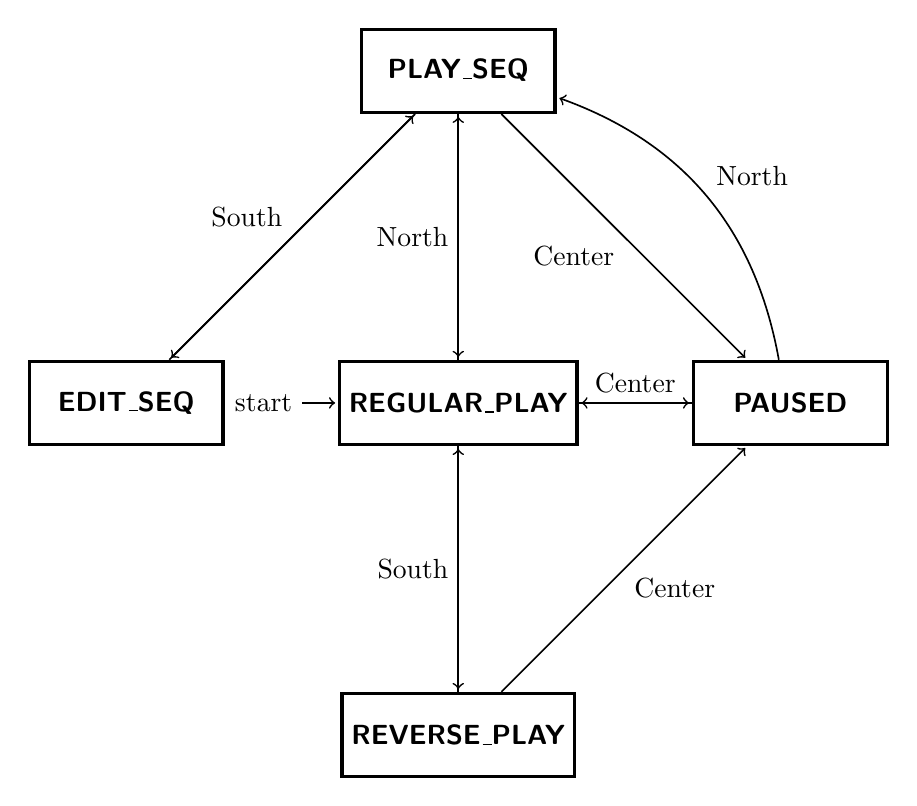
\begin{tikzpicture}[shorten >=1pt, node distance=10cm,on grid, auto, semithick]
	\tikzstyle{state} = [draw, very thick, fill=white, rectangle, minimum height=3em, minimum width=7em, node distance=12em, font={\sffamily\bfseries}]
	\tikzstyle{stateEdgePortion} = [black,thick];
	\tikzstyle{stateEdge} = [stateEdgePortion,->];
	\tikzstyle{edgeLabel} = [pos=0.5, text centered, font={\sffamily\small}];
	
	\node[state,initial](rp) {REGULAR\_PLAY};
	\node[state](revp) [below =of rp]{REVERSE\_PLAY};
	\node[state](p) [right=of rp]{PAUSED};
	\node[state](playseq) [above=of rp]{PLAY\_SEQ};
	\node[state](editseq) [left=of rp]{EDIT\_SEQ};
	
	\path[->]
	(playseq) edge node [swap] {Center} (p)
	edge node [swap] {South} (editseq)
	edge node {} (rp)
	(editseq) edge node {} (playseq)
	(rp) edge node {Center} (p)
	edge [swap] node {South} (revp)
	edge node {North} (playseq)
	(p) edge node {} (rp)
	edge [bend right, swap] node {North} (playseq)
	(revp) edge [swap] node {Center} (p)
	edge [swap] node {} (rp);
	\end{tikzpicture}
\end{center}

The program will print out information as you transition the state machine, edit notes in the sequencer, and modify the tempo.

\subsection{AC97 Controller Hookup}

Take a look at the AC97 controller template provided in \verb|hardware/src/audio/ac97_controller.v|. You will notice that it is a little different from the one used in Lab 5. For one, you will notice that there is a parameter for the system clock frequency which you can use to time the codec reset. Additionally, there are ports that expose the read side of an async FIFO.

Copy over and modify your AC97 controller from Lab 6 so that it holds the codec reset low for the appropriate number of clock cycles depending on the system clock frequency.

Then, if needed, modify your AC97 controller to fetch PCM samples from the async FIFO. On every AC97 frame, you should attempt to fetch a new sample from the FIFO and use it as the PCM data for the left and right channel. If the FIFO is empty, then your AC97 controller should continue playing the last sample it received for the next frame. You should fetch from the FIFO using the \verb|bit_clk|.

After modifying your controller for the new design specs, instantiate it in \verb|ml505top.v|, hook it up to an instance of the async FIFO, and hook the FIFO's write interface into the RISC-V core. Here is the memory map:

\begin{table}[hbt]
	\begin{center}
		\caption{AC97 Controller Memory Map}
		\begin{tabular}{l l l l}
			\toprule
			\textbf{Address} & \textbf{Function} & \textbf{Access} & \textbf{Data Encoding}\\
			\midrule
			32'h80000040 & AC97 FIFO Status & Read & \{31'b0, AC97 FIFO full\} \\
			32'h80000044 & AC97 FIFO Send Sample & Write & \{12'b0, AC97 FIFO din[19:0]\} \\
			32'h80000048 & AC97 Volume Control & Write & \{28'b0, volume\_control[3:0]\}\\
			\bottomrule
		\end{tabular}
	\end{center}
\end{table}

You will notice that you should add a memory mapped register so that the CPU can control the volume. You should be cautious here since metastability issues may arise as the volume control register is clocked by the system clock and is read by the \verb|bit_clk|. In this instance, you can not worry about adding synchronizer elements due to the volume control register changing very infrequently, but this is something to keep in mind.

\subsubsection{AC97 Controller Integration Testbench}
An integration testbench has been provided in \verb|/hardware/src/testbenches/ac97_integration_testbench.v|. The software for this testbench is in \verb|/software/ac97_integration_tb/ac97_integration_tb.c|. 

This testbench performs an end-to-end check of your AC97 controller, the CPU's AC97 FIFO memory map, and the async FIFO. It verifies that all parts of your system can successfully communicate with each other and pass data along. If you look at the software, you will see that the testbench involves sending the PCM samples -50, -49, ..., 49, 50 to the async FIFO, which should then be read and transmitted to the codec by the AC97 controller.

You can run this testbench as usual with \verb|make sim|. This testbench instantiates \verb|ml505top| so you need to have your AC97 controller, AC97 async sample FIFO, and RISC-V core properly hooked up at the top-level.

To interpret the output, view the waveform and plot Slot 3 and Slot 4 of the codec model. Verify that the CPU wrote all the PCM samples to the async FIFO and that the AC97 controller pulled out every sample from the async FIFO and sent it to the codec. Make sure that you verify that the FIFO is empty as soon as PCM sample 50 is pulled from the FIFO, and that once the FIFO is empty, the AC97 controller keeps replaying the last sample that it fetched from the FIFO (50).

A common bug is to make naive assumptions about the async FIFO interface. Remember that the async FIFO is synchronous on both the read and write interface with respect to the read and write clocks. Thus, when reading from the FIFO, if \verb|rd_en| is asserted on a rising read clock edge, the \verb|dout| signal will have the data \textbf{after} the rising edge. This also means that you should check the \verb|empty| condition on the same edge that \verb|rd_en| is asserted, and not on the next cycle.

\subsubsection{AC97 Controller Testing - Tone Program}
We have provided a program in \verb|software/ac97_basic_test/| that sends samples to the AC97 controller via the memory mapped I/O interface. Build and run this program just like \verb|mmult|. Plug in your headphones or speakers to the headphone jack on the board. This program sends a square wave of a certain frequency to the AC97 sample FIFO, and updates the volume register with the state of the DIP switches.

Use the first 4 DIP switches to set the volume. Spin the rotary wheel to change the frequency of the square wave. Press in the rotary wheel to reset the frequency to 440 Hz. Verify that your AC97 controller and async FIFO work as expected.

\subsubsection{AC97 Controller - Piano Program}
To test your AC97 controller, a program is provided that will use your processor to generate sine waves and send them to the AC97 controller via the async FIFO memory map. This program is in \verb|/software/ac97_piano|. Compile and run this program in the same way as the previous ones.

Once you execute \verb|jal 10006000|, you should be able to use your keyboard as a piano and play notes by typing into screen (very similar to lab 6). You will hear the output coming from the headphone jack. To switch octaves, hold down the shift key while playing keys. You may want to look at the keymap in \verb|ac97_piano.c| to figure out what characters map to what notes.

You might have to turn up the volume on your headphones or speakers to hear the output properly.

\subsection{EECS 251A Project Extension - AC97 Mic Input}
\textbf{If anyone in your project group is taking the graduate version of this course, your group will be required to do this section.} This section is optional for project groups where everyone is an undergraduate.

Extend your AC97 controller to be able to read PCM samples from the codec. This is useful if you have a mic connected to the mic jack on the ML505 board and you want to be able to process the input signal. 

To do this, you will want to write some other registers on the AC97 codec to enable the mic input. Specifically, you have to write to the Mic Volume Register (0x0E), Record Select Control Register (0x1A), and the Record Gain Register (0x1C). Take a look at the details in the AD1981B Datasheet in \verb|labs_sp17/docs|.

In addition to enabling the mic input, you will have to modify your AC97 controller to read the \verb|sdata_in| signal coming from the AC97 codec to the FPGA. This serial line has data encoded as AC97 frames, similar to the ones you send out on \verb|sdata_out|. For the details, you should take a look at the AC97 spec in \verb|labs_sp17/docs|, page 33. You will want to sample \verb|sdata_in| on the falling edge of the \verb|bit_clk|. For this section, you are only concerned with the PCM left channel audio (you can ignore the right channel).

You will then need to create another async FIFO instance, but this time with the read interface connected to the CPU and the write interface connected to the AC97 controller. Add ports to your AC97 controller that give it access to the write side of the async FIFO. On every valid AC97 frame, your AC97 controller should write one mic sample to the async FIFO. The processor should be able to access the read interface of the FIFO with the following memory map extensions:

\begin{table}[hbt]
	\begin{center}
		\caption{AC97 Controller Memory Map}
		\begin{tabular}{l l l l}
			\toprule
			\textbf{Address} & \textbf{Function} & \textbf{Access} & \textbf{Data Encoding}\\
			\midrule
			32'h80000050 & AC97 Mic FIFO Status & Read & \{31'b0, empty\} \\
			32'h80000054 & AC97 Mic FIFO Receive Sample & Read & \{12'b0, dout[19:0]\} \\
			\bottomrule
		\end{tabular}
	\end{center}
\end{table}

To finish this section, you will have to write a small C program (very similar to \verb|echo|) that will fetch samples from the AC97 mic FIFO and push the same samples into the AC97 headphone (audio out) FIFO. The program should do this continuously. You should be able to plug in a mic and a pair of headphones and listen to the mic input through your headphones.

\subsection{Checkpoint 2 Deliverables Summary}

\begin{center}
	\begin{tabular}{m{30mm} m{35mm} m{70mm}}
		\toprule
		\textbf{Deliverable} & \textbf{Due Date} & \textbf{Description} \\
		\midrule
		User I/O + FIFOs + AC97 Controller & \audioDueDate \space - In lab checkoff & Demonstrate the working user IO test program and the music streamer program. Explain your testing methodology for the FIFOs and any system level integration testbenches you created. Demonstrate the piano program. \textbf{EECS251A only}: demonstrate mic input to headphone output program. \\
		\bottomrule
	\end{tabular}
\end{center}

\pagebreak

\section{Checkpoint 3 - I2C Master Controller + Video Controller}
In checkpoint three of this project, you will implement a memory mapped I/O interface to a provided I2C master. This will give us access to all I2C devices on the FPGA, including the video controller. Writing to the video controller will allow us to display demo color bars on our VGA output.

We will then build a controller module to handle the Chrontel CH7301C DVI Transmitter Device on our FPGA. This controller will supply the clock timing and logic, allowing us to produce images on our VGA output. We will also generate another block ram to serve as our frame buffer.
 
Finally, we build a simple arbiter and a graphics accelerator that implements the Bresenham line algorithm. This dedicated hardware block will rapidly write to the frame buffer, bypassing the CPU. The arbiter will prioritize the accelerator writes over the CPU writes.
 
Get started by pulling the latest skeleton files from the staff repository: \verb|git pull staff master|.

Here is a block diagram of our entire FPGA design. You should recognize the parts you have already built. It will be helpful to refer back to this to see how things ought to integrate.

\begin{figure}[H]
	\includegraphics[width=\textwidth]{EECS151_Project_Block_Diagram.png}
	\caption{Block Diagram of Entire EECS151 Project, dashed blue line indicates boundary of ml505top}
\end{figure}

\subsection{I2C}
While you will not be implementing an I2C controller, it is helpful to have a brief understanding of I2C.\footnote{For more reading on I2C, see \url{"http://www.nxp.com/documents/user_manual/UM10204.pdf"}}

\begin{figure}[hbt]
\begin{center}
	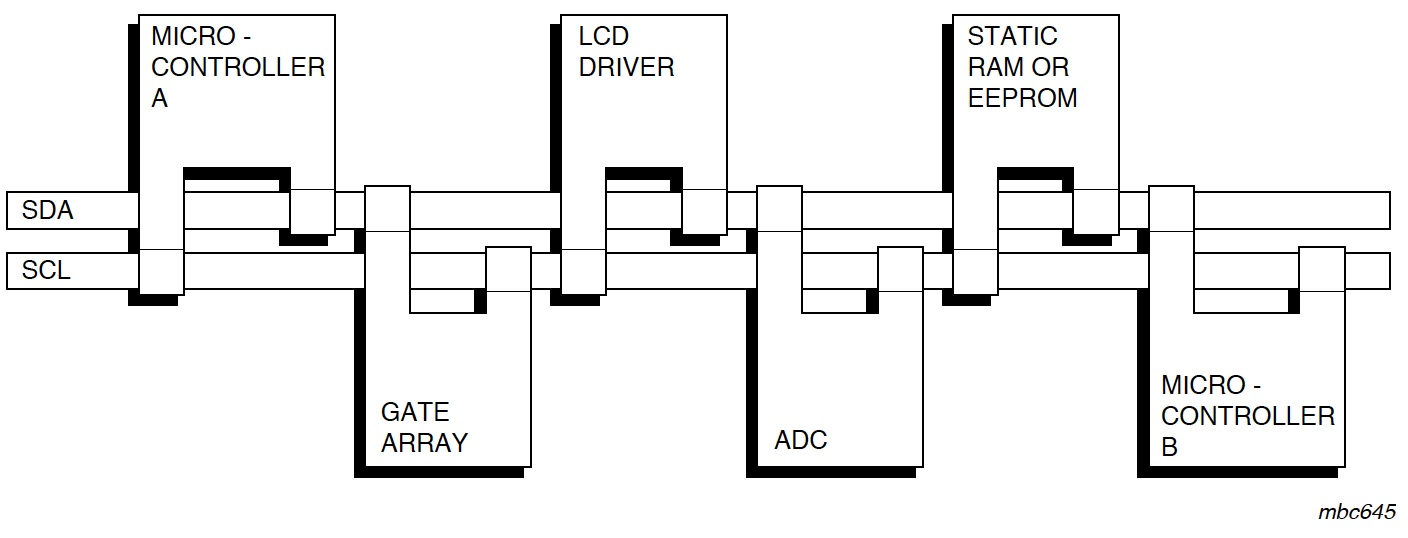
\includegraphics[width=4in]{I2C_example}
	\caption{Example of a multi-master I2C configuration}
	\label{fig:i2c_overview}
\end{center}
\end{figure}

Inter IC or I2C is a simple bidirectional 2-wire serial bus designed by Philips Semiconductor and is a de facto international standard. Multiple devices can connect to the same bus and act as masters or slaves. Unlike the ready-valid interface that we have been using, I2C  reduces the physical complexity of the bus while maintaining flexibility and interoperability. 

The two I2C wires are a data line \verb|SDA| and a clock line \verb|SCL|. Any master device may generate a clock and send data over these shared lines, and the data is free for any device to interpret. The intended slave device will have a specific address encoded, which is used to direct the transaction. The slave also sends acknowledgments back to the master after every byte of data to confirm integrity.

Note that having a shared bus with multiple masters can lead to data collisions when multiple masters attempt to initiate transfers. This is handled in the I2C spec, but is beyond our discussion.

In the simplest terms, an I2C transactions contains 3 steps. First, a given master addresses the slave on the line, and the slave acknowledges. The master then sends register read or write commands to the slave. Finally, the master terminates the transfer.

\subsubsection{Provided I2C}
A complete I2C controller is fairly complex to build, so we have provided you with a complete controller. It uses a set of ready-valid interfaces, which you should be intimately familiar with by now. 

The I2C controller in \verb|hardware/src/video/i2c_controller.v| takes the same 50 MHz clock and reset as the CPU. \verb|i2c_divider| takes in a value to internally divide the 50 Mhz clock to the frequency of \verb|SCL|; we will tie it \verb|0x01F4| to get a 100KHz data rate.

The slave device is normally 7 bits, and the register address, read data, and write data are all normally 8 bits. However, in the provided controller, these registers are 16 bits each in order to pass extra information to the I2C controller. 

\begin{table}[hbt]
	\begin{center}
		\caption{I2C Controller I/O Mapping}
		\label{i2c_ctrl}
		\begin{tabular}{l l l}
			\toprule
			\textbf{Signal} & \textbf{Function} & \textbf{Data Encoding}\\
			\midrule
			i2c\_divider & Clock Divider Setting & \{divisor\} \\
			i2c\_slave\_addr\_unreg & Slave Device Address &  \{8'b0, slave address[6:0], active-low write enable\} \\
			i2c\_reg\_addr\_unreg & Slave Register Address & \{num\_bytes[7:0], register address[7:0]\} \\
			i2c\_wdata\_unreg & Register Write Data & \{num\_bytes[7:0], register write data[7:0]\} \\
			i2c\_rdata & Register Read Data & {8'b0, register read data[7:0]} \\
			i2c\_rdata\_ready, i2c\_rdata\_valid & ready-valid for read data &  \\
			i2c\_ctrl\_ready, i2c\_ctrl\_valid & ready-valid for controller 
		\end{tabular}
	\end{center}
\end{table}

The software will take care of writing the correct data to each register. As with the UART, the CPU simply needs access to the registers, as described in the next section. This information is provided to help with testing.

\subsubsection{Hookup I2C to Memory-Mapped I/O}

Here is the new memory map:
\begin{table}[H]
	\begin{center}
		\caption{Updated Memory Map with I2C}
		\label{i2c_mem_map}
		\begin{tabular}{l l l l}
			\toprule
			\textbf{Address} & \textbf{Function} & \textbf{Access} & \textbf{Data Encoding}\\
			\midrule
			32'h80000100 & I2C status & Read & \{30'b0, i2c\_rdata\_valid, i2c\_ctrl\_ready\} \\
			32'h80000104 & I2C register read data  & Read & \{24'b0, i2c\_rdata\} \\
			32'h80000108 & I2C register address & Write & \{16'b0, i2c\_reg\_addr\} \\
			32'h8000010c & I2C register write data & Write & \{16'b0, i2c\_wdata\} \\
			32'h80000110 & I2C slave address & Write & \{16'b0, i2c\_slave\_addr\} \\
			32'h80000114 & I2C controller trigger & Write & Executes I2C transaction
		\end{tabular}
	\end{center}
\end{table}

You need to create registers in your CPU for \verb|i2c_reg_addr|, \verb|i2c_wdata|, and \verb|i2c_slave_addr|. You should pulse \verb|i2c_ctrl_valid| when a write is performed to the I2C control trigger address. You should pulse \verb|i2c_rdata_ready| when a read is performed from the I2C register read data address.

Modify \verb|Riscv151.v| to include these memory mapped registers.

We will also have to modify \verb|ml505top.v| and the UCF to include the I2C lines. Be sure the following are added to your top module and the UCF. Otherwise, run \verb|git pull staff master|. 

\begin{table}[hbt]
	\begin{center}
		\caption{Top Module Connections for I2C}
		\label{i2c_ucf}
		\begin{tabular}{l l l}
			\toprule
			\textbf{Name} & \textbf{FPGA Loc} & \textbf{IO Standard}\\
			\midrule
			IIC\_SCL\_VIDEO & U27  & LVCMOS18 \\
			IIC\_SDA\_VIDEO & T29 & LVCMOS18 
		\end{tabular}
	\end{center}
\end{table}


\subsubsection{I2C Testbench}
To help you verify that the I2C controller is hooked up properly, we have provided an I2C slave model. This model will print out information about the transaction times, slave address, device register, register data, transaction acknowledgement, etc.

The testbench files are located in \verb|hardware/src/testbenches/i2c_integration_testbench.v|, \verb|hardware/sim/i2c_integration_testbench.do|, and \verb|software/i2c_integration_tb|.

To run the testbench,
\begin{enumerate}
	\item Run \verb|make| in \verb|software/i2c_integration_tb|
	\item Run \verb|make CASES=tests/i2c_integration_testbench.do| in \verb|hardware/sim|
	\item Observe the testbench output; it should correspond to the transactions enumerated in the software. Specifically:
	\begin{enumerate}
		\item An I2C read from slave 0x76, reg 0x01
		\item An I2C write to slave 0x76, reg 0x34, data 0xfa
		\item an I2C write to slave 0x76, reg 0x85, data 0x39
	\end{enumerate}
	\item Verify in Modelsim that the I2C read ended with \verb|i2c_rdata| of 0xa5 and that your CPU pulsed \verb|i2c_rdata_ready| after \verb|i2c_rdata_valid| was asserted
	\item Verify that the slave model saw the two I2C write commands as they were written in the software
\end{enumerate}

\subsubsection{I2C Testing on the FPGA}
Once things work in simulation, \verb|make| and \verb|make impact| your design to the FPGA. Load the \verb|graphics| program in \verb|software/graphics| into your CPU using \verb|coe_to_serial| as usual, and \verb|jal| to it from the BIOS.

When you see the \verb|graphics >| prompt, issue the command \verb|setup|. The program will attempt to perform I2C write commands to the Chrontel Video Chip to configure it properly. Looking at the \verb|graphics.c| file in \verb|software| you can see that it performs an I2C read after every I2C write and prints out the data it got in the \verb|i2c_setup()| function. You need to verify that the values that were read over I2C match the values that were written to the chip; the values are printed out.

As an additional check, at the end of the \verb|i2c_setup()| function, the Chrontel chip's Version and Device IDs are printed out. Look up those values in the Chrontel chip's datasheet (in \verb|useful_docs|) and verify that they match what was printed.

If all these things look good, then your I2C controller is properly hooked up!

\subsection{Frame Buffer}
The video controller has to continuously send data to the Chrontel video chip: pixel by pixel. It needs a place from where to fetch this pixel data. Also, our CPU needs to be able to control whether a given pixel is on or off. The place we store this pixel data is called the frame buffer. We are targeting an output resolution of 1024 x 768, which gives us a total of 786432 pixels.

To that end, we will generate a 786432x1 block RAM, where each line stores a single pixel's data. We are only use 1 bit per pixel (i.e. black or white), in the interest of keeping the FPGA design small in area, and because we have a limited amount of memory on the FPGA.

Each 1-bit line of this RAM will be assigned a byte address. Each byte will be either high or low, representing a light or dark pixel. The pixels will be ordered left to right, then top to bottom. This matches the VGA pixel order. 

The CPU will be able to write to the frame buffer just like it writes to the data memory. Thus we need to reserve an address space for it. To make space for all 786432 pixels, we will reserve the addresses 0x90000000 through 0x900BFFFF for the frame buffer.

\begin{table}[hbt]
	\begin{center}
		\caption{Framebuffer Memory Map Additions}
		\label{frame_buffer}
		\begin{tabular}{l l l l}
			\toprule
			\textbf{Address} & \textbf{Function} & \textbf{Access} & \textbf{Data Encoding}\\
			\midrule
			32'h900XXXXX & Frame Buffer & Write & \{31'b0, data\} \\
		\end{tabular}
	\end{center}
\end{table}

For (x, y) coordinates where $x \in {0, 1, ... 1023}$ and $y \in {0, 1, ..., 767}$ the memory address becomes \verb|0x90000000 + (y << 10) + x|. You can assume that all writes to the framebuffer will be in the form of \verb|sb| (store byte) instructions.

The framebuffer's block RAM needs to be built. To do this:
\begin{enumerate}
	\item Go to \verb|hardware/src/video/framebuffer_ram|
	\item Run \verb|./build|
	\item Open up \verb|block_mem_1x786432.v| and make sure you have a dual ported block RAM that was generated
	\item The module you should instantiate wraps the block RAM and is located in\\ \verb|hardware/src/video/frame_buffer_1_786432.v|.
\end{enumerate}

You only need to do this once.

\subsection{Chrontel Chip}
The Chrontel CH7301C DVI Transmitter Device on the ML505 board can receive digital pixel data over a parallel bus from the FPGA, and it can output a DVI video signal to a monitor. It can also drive an analog VGA output when VGA-bypass mode is enabled. The datasheet for this chip can be found in the \verb|useful_docs| folder.

\begin{figure}[H]
\begin{center}
	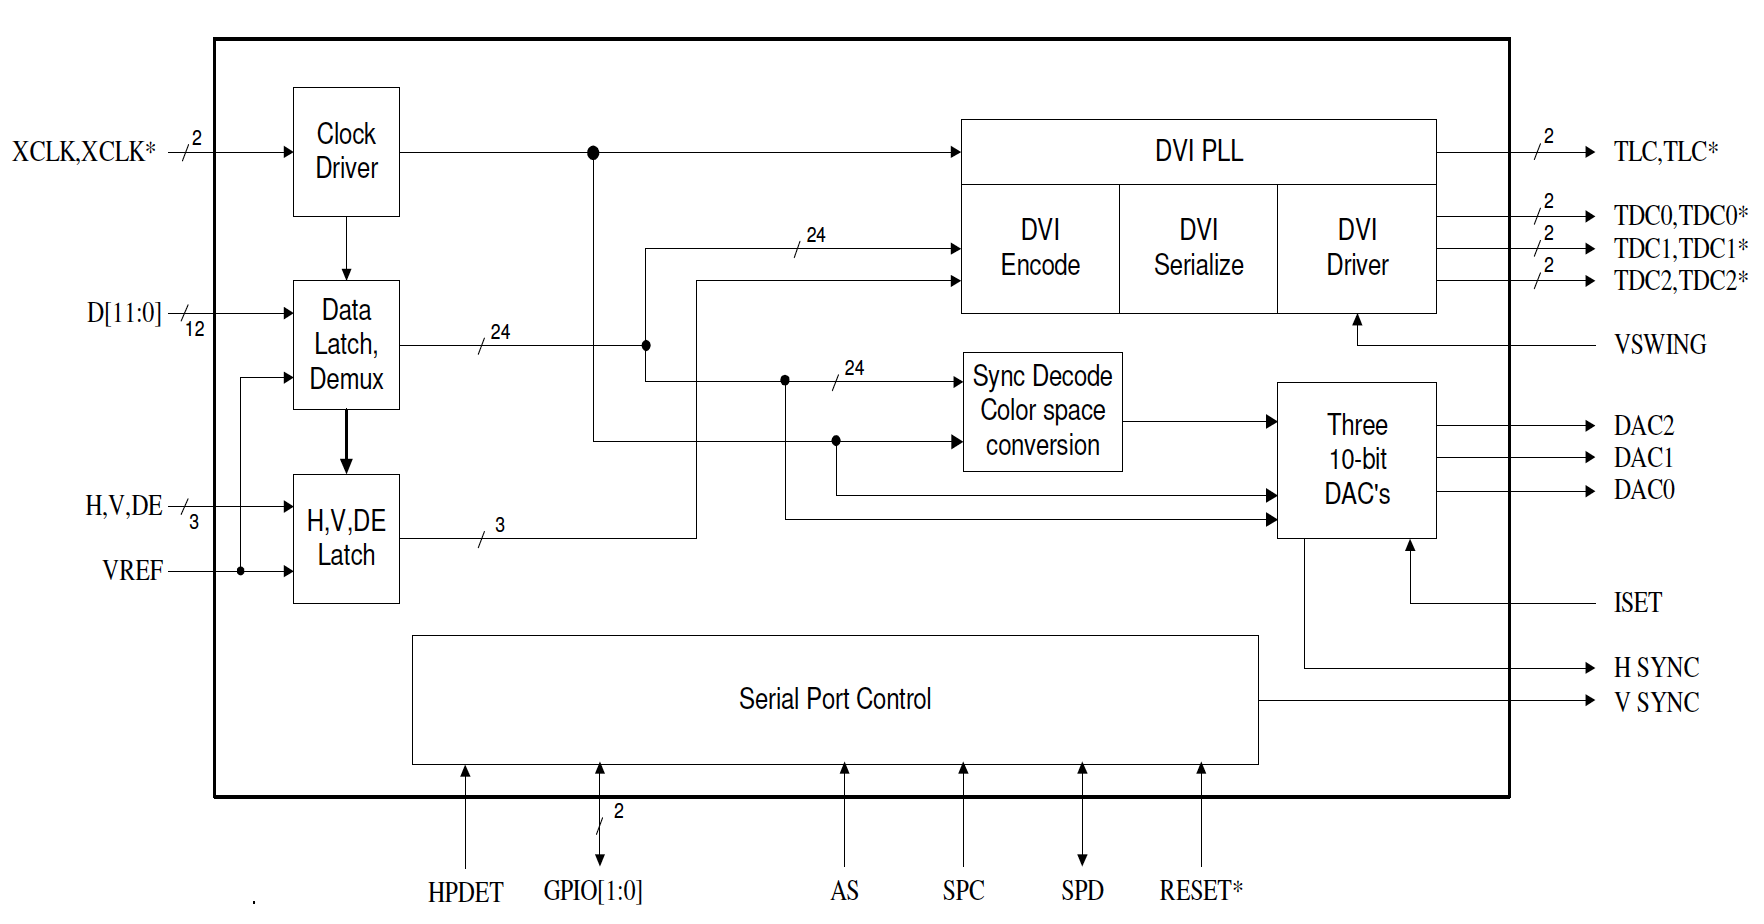
\includegraphics[width=6.5in]{dvi_block}
	\caption{Chrontel chip block diagram - from datasheet}
	\label{fig:dvi_block}
\end{center}
\end{figure}

\subsubsection{Control Registers}
Just like the AC97 codec, the Chrontel video chip has many internal registers that configure how it operates. The Chrontel chip receives read and write register commands over I2C, which you tested in the previous section. Below is a reduced list of the registers to write to. See the Chrontel datasheet for more details.

\begin{table}[H]
	\begin{center}
		\caption{Chrontel Control Registers}
		\label{chrontel_registers}
		\begin{tabular}{l l l l}
			\toprule
			\textbf{Address} & \textbf{Function} & \textbf{Default} & \textbf{Desired} \\
			\midrule
			8'h21 & DAC Control & 8'h00 & 8'h09 \\
			8'h33 & Charge Pump Control & 8'hE4 & 8'h08 \\
			8'h34 & DVI PLL Divider & 8'h16 & 8'h16 \\
			8'h36 & DVI PLL Filter & 8'h00 & 8'h60 \\
			8'h48 & Test Pattern & 8'h18 & 8'h19 \\
			8'h49 & Power Management & 8'h01 & 8'hC0 \\
			8'h56 & DVI Sync Polarity & 8'h00 & 8'h00 \\
			8'h1F & Input Data Format & 8'h00 & 8'h83 
		\end{tabular}
	\end{center}
\end{table}

These registers will be set via the \verb|graphics| program; it is all done for you. The slave device address for the Chrontel chip is 0x76.

\subsubsection{Chrontel Chip I/O}
The Chrontel chip takes several inputs that represent video data. Here is a list of relevant signals (they are all outputs from the FPGA and inputs to the chip):

\begin{itemize}
	\item \textbf{DVI\_XCLK\_N, DVI\_XCLK\_P} - A differential clock input to the Chrontel chip. The chip uses this clock to sample the data lines. For achieving a 1024 x 768 resolution with a 60 Hz refresh rate, this clock is set at 65 Mhz. It is generated and driven for you in \verb|ml505top| and \verb|src/video/dvi_controller.v|.
	
	\item \textbf{DVI\_RESET\_B} - An active-low reset input to the Chrontel chip. This is permanently held high in our design since we will be resetting the chip over I2C rather than using this signal.
	
	\item \textbf{DVI\_D [11:0]} - The data bus representing the color data for a given pixel. The details on how to drive this bus can be found on page 7 and page 10 of the datasheet. We are using IDF (input data format) = 3 in our controller. This bus is latched by the chip on both the rising and falling edges of the \verb|XCLK|.
	
	\item \textbf{DVI\_V} - Vertical sync input to the Chrontel chip. Should be driven \underline{active-low}. Tells the chip when a new video frame is about to start.
	
	\item \textbf{DVI\_H} - Horizontal sync input to the Chrontel chip. Should be driven \underline{active-low}. This tells the chip when a new horizontal line is about to start.
	
	\item \textbf{DVI\_DE} - Data enable input to the Chrontel chip. The \verb|DVI_D| bus' data is valid for the chip to latch when this signal is asserted \underline{active-high}.
\end{itemize}

All these signals are driven using the \verb|dvi_controller| located in \verb|src/video/dvi_controller.v|. You will develop this module in this checkpoint.

\subsection{Building the DVI Controller}
To send video data to the Chrontel chip, we need to strobe the \verb|DVI_V|, \verb|DVI_H|, \verb|DVI_DE|, and \verb|DVI_D[11:0]| signals appropriately. The way to drive these signals comes from the VGA timing spec.

\subsubsection{Timing}

\begin{figure}[H]
\begin{center}
	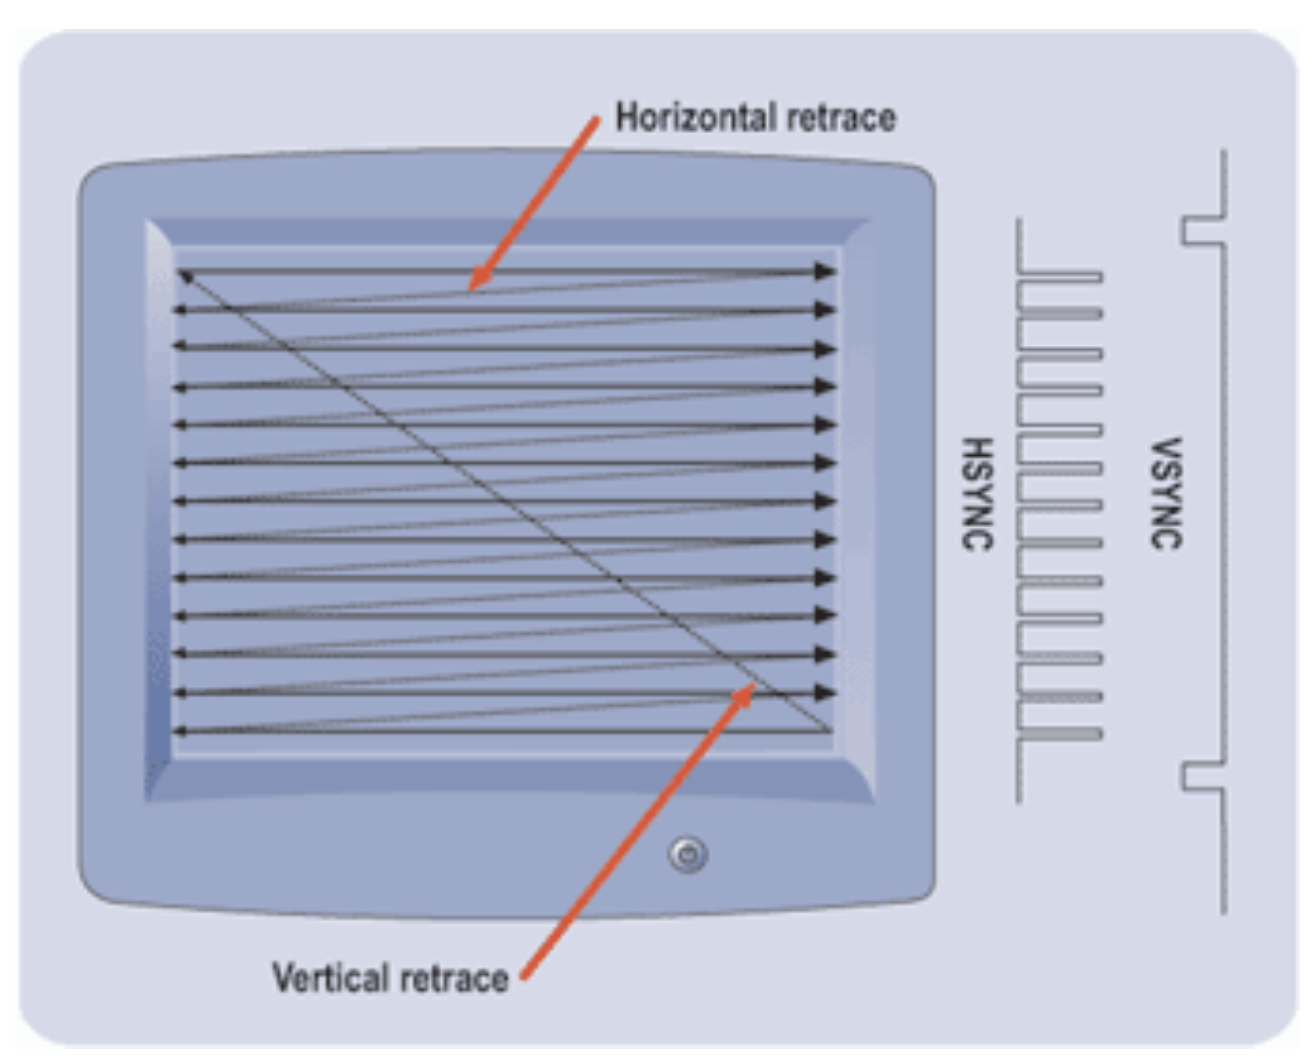
\includegraphics[height=4cm]{vga_overview}
	\caption{VGA timing scheme}
	\label{fig:vga_overview}
\end{center}
\end{figure}

The VGA protocol uses a strict clock synchronization protocol to draw each pixel on screen from left to right, then top to bottom. It uses two synchronization signals: a horizontal sync and a vertical sync. The vertical sync signal denotes the beginning of a image, or frame. The horizontal sync signal denotes the beginning of each horizontal line of pixels. Both signals are \underline{active low}.

For each of sync signals, there are 4 major components: the sync pulse, the back porch immediately following, the display active time, and the front porch before the next sync signal. Only during the display active time do we want to be sending valid data to the Chrontel chip.

\begin{figure}[H]
\begin{center}
	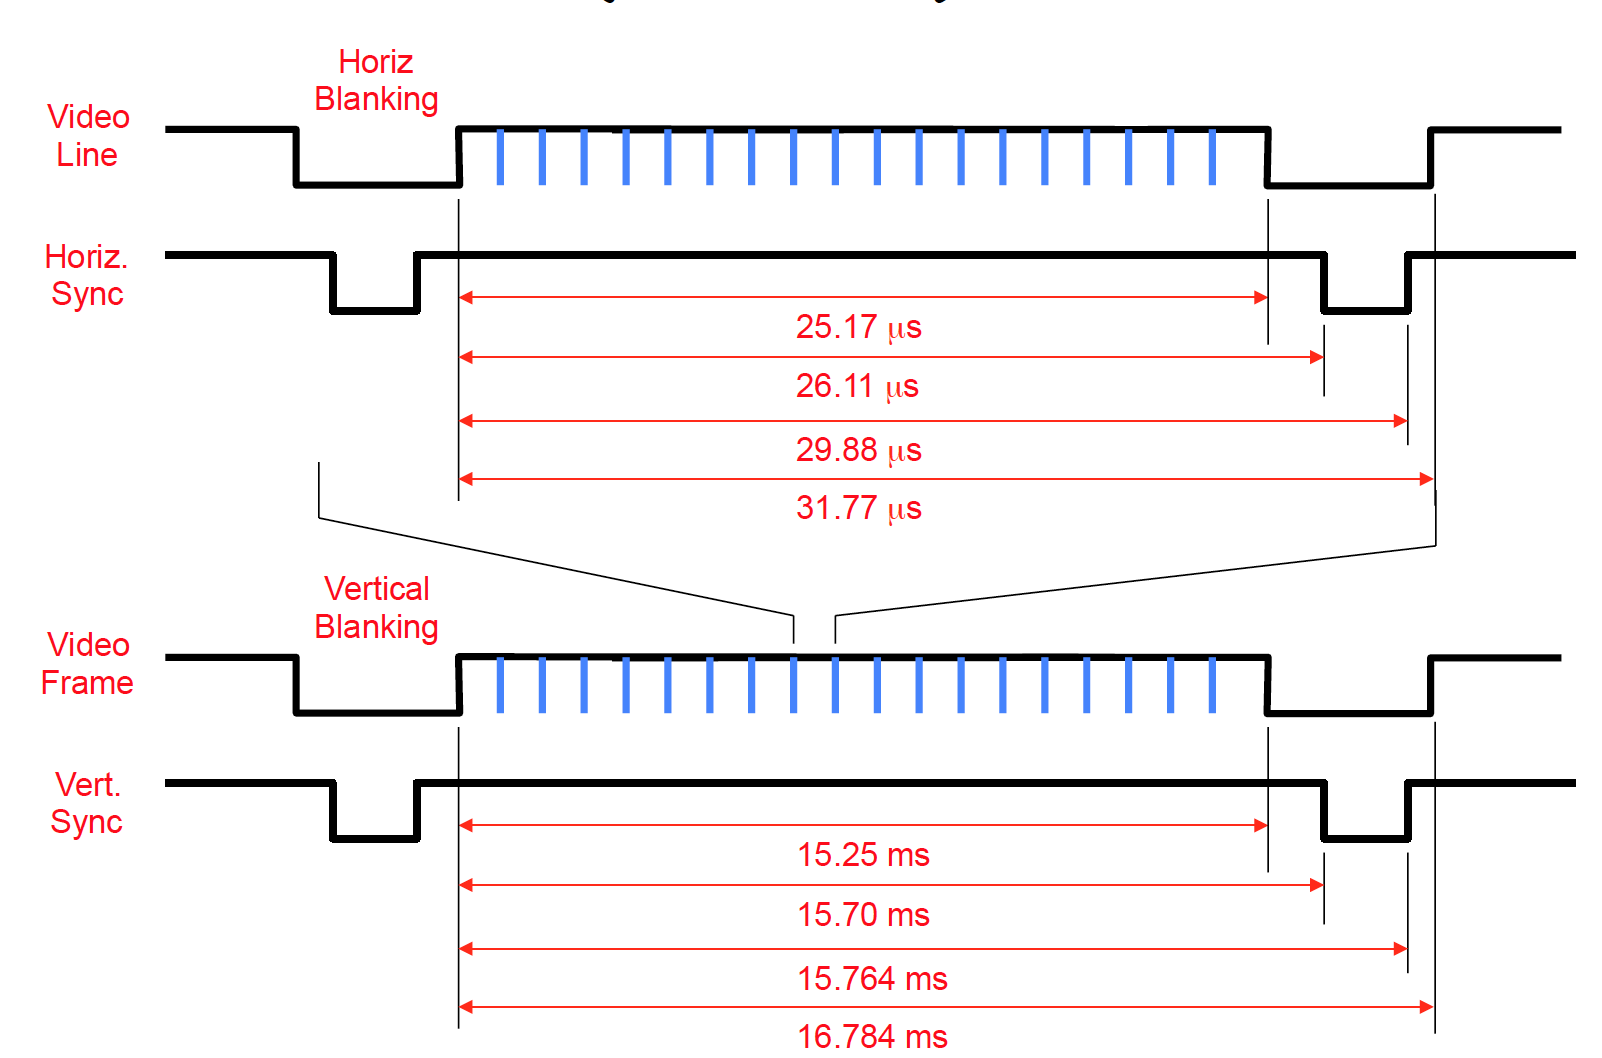
\includegraphics[width=4in]{vga_timing}
	\caption{VGA timing detailed}
	\label{fig:vga_timing}
	
	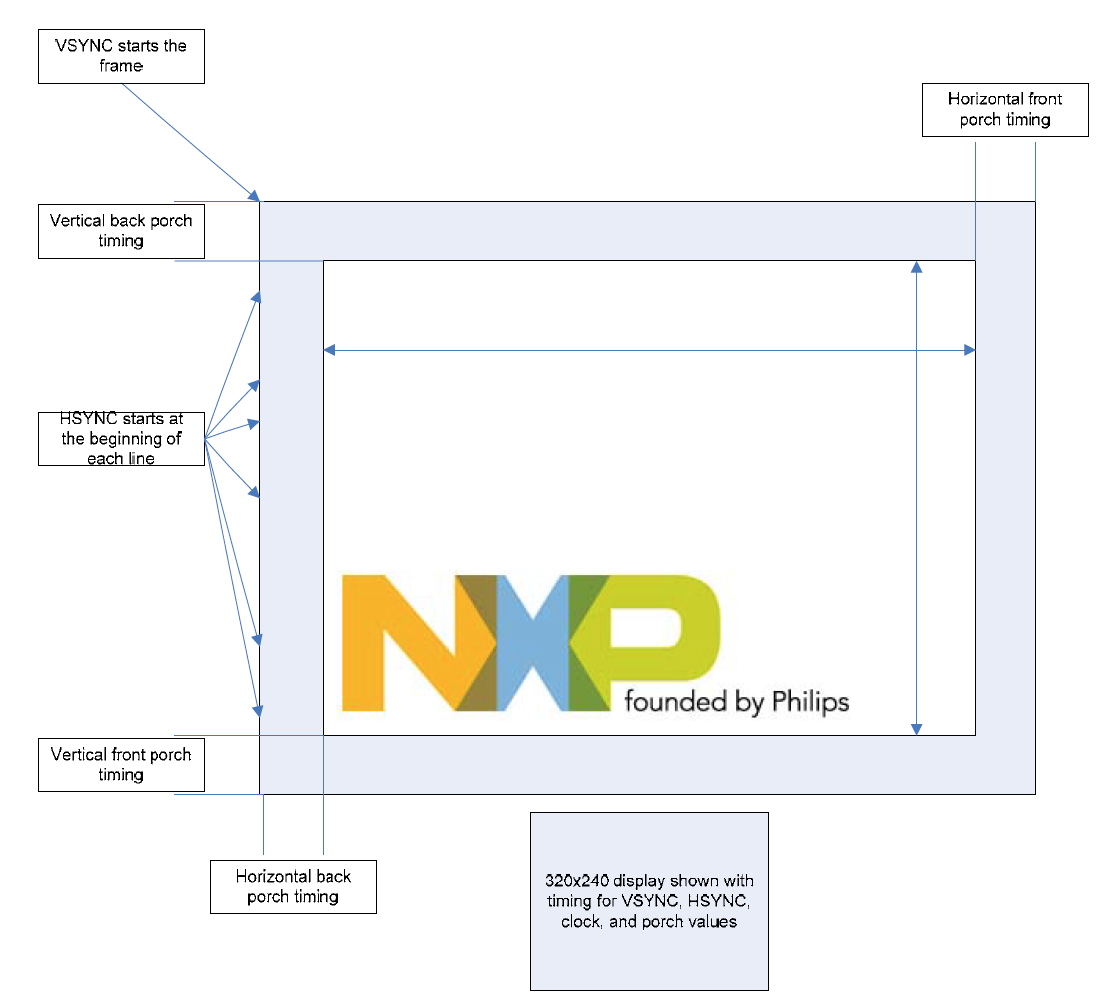
\includegraphics[width=4in]{vga_frame}
	\caption{VGA frame with timing}
	\label{fig:vga_frame}
\end{center}
\end{figure}

Note that during the vertical sync pulse, the horizontal sync pulse should be inactive as to not denote the start of a line.

\subsubsection{Parameters}
We will be using a resolution of 1024 x 768 at a 60 Hz refresh rate. This will require us to use a 65 MHz clock and the following timing parameters.

\begin{table}[H]
	\begin{center}
		\caption{VGA Timing for 1024 x 768 at 60 Hz (XGA)}
		\label{vga_timing_table}
		\begin{tabular}{l l l}
			\toprule
			\textbf{Name} & \textbf{Pixel/Line Length} & \textbf{Real Time}\\
			\midrule
				  H Sync Pulse    &  136 & 2.09 us \\
				  H Back Porch    &   160 & 2.46 us \\
				  H Visible Area    &   1024 & 15.7 us \\
				  H Front Porch    &   24 & 0.37 us \\
			\midrule
				  V Sync Pulse    &  6 & 124 us \\
				  V Back Porch    &   29 & 600 us \\
				  V Visible Area    &   768 & 15.9 ms \\
				  V Front Porch    &   3 & 62 us \\
		\end{tabular}
	\end{center}
\end{table}

Here is how the sync and DE signals should be driven:

\begin{enumerate}
	\item At the start of the frame, assert \verb|DVI_V| for \verb|V Sync Pulse| horizontal lines (each horizontal line consists of 1344 pixels or clock periods)
	\item Don't assert any signals for \verb|V Back Porch| horizontal lines
	\item For \verb|V Visble Area| lines perform the following sequence:
	\begin{enumerate}
		\item Assert \verb|DVI_H| for \verb|H Sync Pulse| clock periods
		\item Don't assert any signals for \verb|H Back Porch| clock periods
		\item Assert \verb|DVI_DE| and place the pixel data on \verb|DVI_D[11:0]| for \verb|H Visible Area| clock periods
		\item Don't assert any signals for \verb|H Front Porch| clock periods
	\end{enumerate}
	\item Don't assert any signals for \verb|V Front Porch| horizontal lines
	\item Start again at step \#1 to send the next video frame
\end{enumerate}

We will be using one-bit color: either black or "white". We will tint our "white" a slight blue. This implementation is simple to expand to 3-color RGB and to multi-bit RGB, with 5-bits of color each. This is not a requirement of the project, but you are welcome to try it for extra credit.

\subsubsection{Data Formatting}
The Chrontel chip supports multiple schemes for transferring color information over the 12-bit \verb|DVI_D| bus. We will be using IDF = 3 with "XCLK 1x" as listed in the datasheet. This provides us with up to 15-bit RGB color. For simplicity however, we are using only 1-bit color. We must translate our 1 bit to 15 bits. Use the following scheme. It will yield a light blue tint for "1," and black for "0."

\begin{table}[hbt]
	\begin{center}
		\caption{Colors}
		\label{colors}
		\begin{tabular}{l l l l}
			\toprule
			\textbf{Pixel Value} & \textbf{Red} & \textbf{Green} & \textbf{Blue} \\
			\midrule
			1 & 5'b11000 & 5'b11000 & 5'b11111 \\
			0 & 5'b0  & 5'b0 & 5'b0 \\
		\end{tabular}
	\end{center}
\end{table}

\begin{figure}[hbt]
\begin{center}
	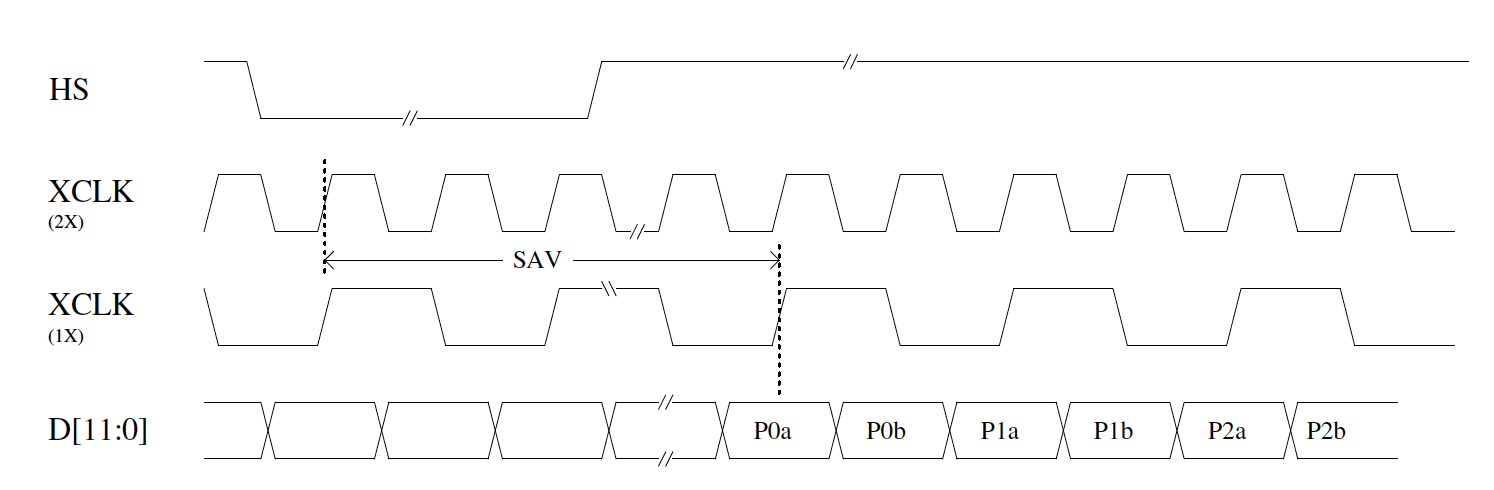
\includegraphics[width=6.5in]{chrontel_data_timing}
	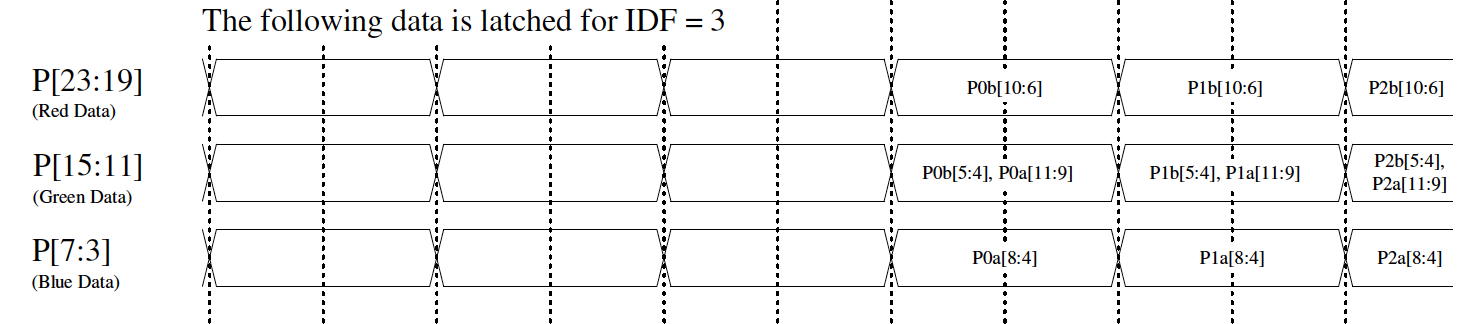
\includegraphics[width=6.5in]{idf3}
	\caption{Chrontel Data Timing}
	\label{fig:chrontel_data_timing}
\end{center}
\end{figure}

You will note that the 12-bit data input changes on both rising and falling clock edges. To support this, we will be buffer the rising edge data and the edge phase data with an ODDR buffer primitive. This buffer will update on both clock edges and can take two different inputs. Look at the provided skeleton in \verb|src/video/dvi_controller.v| for the instantiations of the ODDR primitives.

\subsubsection{Hookup}

You will need to instantiate your DVI controller and the framebuffer in \verb|ml505top|. You can add additional ports to your CPU so it can write to the framebuffer. In \verb|ml505top| the reset signal to be used with your DVI controller should be \underline{video\_reset}, NOT \verb|reset|.

\subsection{DVI Controller Testing}

Your task is to build a controller that reads from the frame buffer and provides all the necessary signals for the Chrontel chip. This includes the color data, the vertical and horizontal sync signals, the differential XCLK as shown in the Chrontel data timing diagram, and the data enable signal. We have provided you a skeleton in \verb|src/video/dvi_controller.v| to get started.

\subsubsection{DVI Controller Testbench}
Once you have made a first pass at the \verb|dvi_controller|, you can try running the \verb|dvi_controller_testbench| located in \verb|hardware/src/testbenches/dvi_controller_testbench.v|. This testbench writes color bars to the instantiated framebuffer and lets your DVI controller pull pixel data from the framebuffer and transmit it. We have also written a \verb|ch7301_model| which you can find in\\ \verb|hardware/src/testbenches/models/video_codec_model.v|. This model will perform timing checks on your sync signals and will print out the pixel data it receives from your controller.

When running this testbench for the first time, you might see a ton of error output indicating various timing inconsistencies. Don't panic; start at the first timing violation and rerun the testbench when you think you have solved an issue. It is common for this model to print out many errors due to the strict timing bounds it enforces.

In reality, when running your controller on the FPGA, the Chrontel chip is far more lenient towards timing imperfections so if you see timing discrepancies within a few nanoseconds, or even up to 16 nanoseconds, the controller will likely still work on the FPGA. Please ask a TA if you want to confirm whether it is OK to ignore an almost OK timing discrepancy.

As the testbench runs, the \verb|video_codec_model| will write to a file at \verb|hardware/sim/build/video_data.txt|. The text in this file can be converted into an image by running this in \verb|hardware/sim|:

\begin{minted}{bash}
python video_data_to_images.py build/video_data.txt
\end{minted}

This script may take up to 30 seconds to run. Once it does you will see a folder called \verb|video_frames|. In this folder, you can run \verb|eog frame01.png| to open the image for viewing. You want to manually verify that the image looks like this:

\begin{figure}[H]
	\centerline{
\includegraphics[height=4cm]{dvi_controller_testbench_output.png}}
\end{figure}

Each color bar should be 32-pixels high and they should alternate between light and dark. You should use the Measure tool in GIMP to verify this. Right click on the image when open in \verb|eog|, then click Open With $\rightarrow$ GIMP. In GIMP use the Measure tool (Shift + M) by clicking and dragging to verify the height of the color bars.

\subsubsection{DVI Controller Integration Testbench}
Once your color bars look good, let's test the DVI controller and framebuffer's interaction with your CPU. The integration testbench consists of 3 files:

\begin{enumerate}
	\item \verb|hardware/src/testbenches/dvi_controller_integration_testbench.v|
	\item \verb|hardware/sim/tests/dvi_controller_integration_testbench.do|
	\item \verb|software/dvi_controller_testbench/dvi_controller_testbench.c|
\end{enumerate}

Run this testbench as usual once you have hooked up the framebuffer and DVI controller in \verb|ml505top| and to your CPU's memory map. The software running on the CPU will run a function to draw a line from the top left to bottom right of the frame. This testbench will take longer to execute than the simple block-level testbench. Once it is does, you can create an image from the \verb|video_data| and check to see if a line has been drawn by your CPU. It should look like this (might have to zoom in to see the line):

\begin{figure}[H]
	\centerline{
\includegraphics[height=4cm]{dvi_controller_integration_testbench_output.png}}
\end{figure}

\subsubsection{Testing on the FPGA!}

Once all these testbenches look good \verb|make| and \verb|make impact| your design as usual. Connect the DVI cable from a monitor to the ML505's DVI port; you may have to unplug the monitor from a workstation.

Put the \verb|graphics| program on your FPGA using \verb|coe_to_serial| as usual. Once you \verb|jal 10006000| to it and can see the \verb|graphics >| prompt, you have access to these commands.

\begin{enumerate}
	\item \textbf{setup} - You should run this to configure the Chrontel chip over I2C
	\item \textbf{test\_pattern} - This will configure the Chrontel chip to output a color bar test pattern over the video cable. To go back to framebuffer fetch mode run 'setup' again.
	\item \textbf{fill} [0/1] - This will fill the framebuffer with either 0s or 1s.
	\item \textbf{swline} [0/1] x0 y0 x1 y1 - This will draw a line of color 0 or 1 from (x0, y0) to (x1, y1) using the CPU.
	\item \textbf{pixel} [0/1] x y - This will draw a single position at coordinate (x, y). This is useful for checking that all corners of the video frame can be written to.
	\item \textbf{exit} - Return to BIOS.
\end{enumerate}

\subsubsection{AC97 Visual Piano}
We have written a piano program which uses the DVI controller to display a live view of the waveform being sent to the AC97 controller. It can be found in \verb|software/ac97_piano_visual|.

To use this program:
\begin{enumerate}
	\item Load and jal to the \verb|graphics| program. Execute the 'setup' command.
	\item Load and jal to the \verb|ac97_piano_visual| program. Pressing a key should play a piano note through the headphone jack.
	\item You can spin the rotary wheel to change the 'update rate/decimation factor' that's used to send the waveform to the framebuffer. Spinning the wheel left will 'zoom in' and spinning the wheel right will 'zoom out'. Pushing the wheel in will reset the 'decimation factor' to the default value.
	\item You should be able to see how pressing a key with a higher note pitch results in a higher frequency sine waveform.
\end{enumerate}

\subsection{Hardware Accelerated Line Drawer (Optional)}
This section is optional for checkpoint 3. If you choose to do it, you will be awarded at least 2\% extra credit for the project grade.

\subsubsection{Line Drawing}
We have included a skeleton accelerator in \verb|hardware/src/video/accelerator.v|. The purpose of this module is to receive a 'line draw' command from the CPU and then execute the correct pixel writes to the framebuffer to draw a line. The \verb|accelerator| should be clocked with the \verb|cpu_clk_g|.

You should modify this module to implement Bresenham's Algorithm. You can find some helpful slides here: \url{https://inst.eecs.berkeley.edu/~cs150/fa10/Lab/CP3/LineDrawing.pdf}. 

You should implement a ready/valid interface using the \verb|RX_ready| and \verb|RX_valid| signals. When \verb|RX_valid| is pulsed by the CPU, you should register \verb|x0,y0,x1,y1,color| internally and should pull \verb|RX_ready| low until the line is written to the framebuffer.

\subsubsection{Arbiter}
With the addition of the \verb|accelerator|, the \verb|framebuffer| now has write contention between the CPU and the \verb|accelerator|. Since the \verb|framebuffer| only has 1 write port, only the CPU or the \verb|accelerator| can write to it on a given clock cycle. We resolve this issue using an arbiter. An implementation is provided for you in \verb|hardware/src/video/arbiter.v|.

Our \verb|arbiter| is very simple; it always prioritizes the requests of the \verb|accelerator| over the CPU. You will use the \verb|arbiter| to hook the \verb|accelerator| and the CPU to the framebuffer in \verb|ml505top|.

\subsubsection{Hookup + Testing}
You should modify \verb|Riscv151.v| and/or \verb|ml505top.v| to instantiate your \verb|framebuffer| and \verb|arbiter|.

You should create memory-mapped registers for \verb|x0,x1,y1,y0,color,fire| and you can decide what addresses they should map to. When a write to the \verb|fire| is performed, the \verb|RX_valid| signal should be pulsed for one cycle.

To test the \verb|accelerator| you can modify the software in \verb|software/dvi_controller_testbench| to write to your memory mapped registers and trigger a line drawing. Then the DVI controller and model should function as usual. You can add to the memory map in \verb|software/151_library/memory_map.h| if you want.

\subsubsection{Extend Graphics Program}
Once your accelerator works in simulation, you should extend the \verb|graphics| program to use your accelerator for drawing lines. In \verb|graphics.c|, add a command called 'hwline' which takes the same arguments as 'swline' but uses your accelerator instead of the CPU to draw the line. Now, test it on the FPGA.

\subsection{Checkpoint 3 Deliverables Summary}

\begin{center}
	\begin{tabular}{m{30mm} m{35mm} m{70mm}}
		\toprule
		\textbf{Deliverable} & \textbf{Due Date} & \textbf{Description} \\
		\midrule
		I2C memory map + VGA controller + line drawing accelerator & \ethernetDueDate \space - \dueDateTime & Demonstrate a working VGA color bar test. Demonstrate line or image drawing from both the CPU and the accelerator. Demonstrate the AC97 visual piano. \\
		\bottomrule
	\end{tabular}
\end{center}

\pagebreak

\section{Final Checkpoint - Optimization}
This optimization checkpoint is lumped with the final checkpoint and the checkoff will occur at the same time. This part of the project is designed to give students freedom to implement the optimizations of their choosing to improve the performance of their processor.

The general optimization goal for this project is to achieve maximal performance on the \verb|mmult| program, as defined by the 'Iron Law' of Processor Performance.

\begin{equation*}
\frac{\text{Time}}{\text{Program}} = \frac{\text{Instructions}}{\text{Program}} \times \frac{\text{Cycles}}{\text{Instruction}} \times \frac{\text{Time}}{\text{Cycle}}
\end{equation*}

Your goal is to minimize the execution time of \verb|mmult|. The number of instructions is fixed, but you have freedom to change the CPI and the CPU clock frequency. Often you will find that you will have to sacrifice CPI to achieve a higher clock frequency, but there also will exist opportunities to improve one or both of the variables without compromises.

\subsection{Clock Generation Info + Changing Clock Frequency}
Open up \verb|ml505top.v|. You will notice a top level input called \verb|USER_CLK|. This signal comes from a crystal on the ML505 board and it comes into our FPGA design. It is a 100 Mhz clock signal, which we will use to derive our CPU clock.

Scrolling down a little further, you will see an instantiation of \verb|PLL_BASE|, which is a PLL (phase locked loop) primitive on the FPGA. This is a circuit that lets us create a new clock from a known clock with a user-specified multiply-divide ratio. 

The \verb|CLKIN| input clock of the PLL. is driven by the 100 Mhz \verb|user_clk_g| (buffered \verb|USER_CLK|). The PLL multiplies the frequency of this input clock by the \verb|CLKFBOUT_MULT| parameter, which is set to 6. Thus, internally, the PLL creates a 600 Mhz clock. Then, this multiplied clock is divided by the \verb|CLKOUT0_DIVIDE| parameter. In our case, this parameter is set to \verb|600_000_000 / CPU_CLOCK_FREQ| and \verb|CPU_CLOCK_FREQ = 50_000_000|. Thus our divide parameter is 12. Finally, the multiplied and divided clock ($\times 6 \div 12 = \frac{1}{2}$) shows up at the \verb|CLKOUT0| output clock of the PLL, which is connected to \verb|cpu_clk|. The \verb|cpu_clk| is buffered and \verb|cpu_clk_g| is used in our CPU and other modules.

Take a look at the \verb|CPU_CLOCK_FREQ| parameter at the top of \verb|ml505top|. This sets the clock frequency we want to synthesize from the 100 Mhz \verb|USER_CLK| to be used in the rest of our design. You can alter this parameter to change the CPU clock frequency, but it can't be set arbitrarily, and there are a few caveats. You can only set this value to an integer divisor of 600 Mhz, unless you change the multiplication parameter in the PLL. A few frequencies to try are: 60 Mhz, 75 Mhz, and 100 Mhz. You can also try frequencies in the middle and even adjust the multiply parameter for more variety.

\subsection{Critical Path Identification}
Begin by pulling the latest skeleton files from the staff repository: \verb|git pull staff master|. After running \verb|make|, your FPGA design will be placed and routed, and timing analysis will be performed to determine the critical path(s) of your design. The timing tools will automatically figure out the CPU clock timing constraint based on the multiply-divide ratio you used in your PLL. 

To see the critical path run \verb|make report|, and click on \verb|Post-PAR Static Timing Report| in the list on the left. You are interested in the timing paths for \verb|cpu_clk_g| which is the clock used by your CPU and the rest of your design.

Perform a CTRL+F on \verb|TS_cpu_clk| and you will come upon a section like this in your report:

\begin{minted}[breaklines]{text}
Timing constraint: TS_cpu_clk = PERIOD TIMEGRP "cpu_clk" TS_USER_CLK / 0.5 HIGH 
50%;
For more information, see Period Analysis in the Timing Closure User Guide (UG612).

73245958 paths analyzed, 6219 endpoints analyzed, 0 failing endpoints
0 timing errors detected. (0 setup errors, 0 hold errors, 0 component switching limit errors)
Minimum period is  19.897ns.
\end{minted}

This section indicates the start of the timing report for the CPU clock. It will tell you how the timing constraint for the \verb|cpu_clk| was derived from the \verb|TS_USER_CLK| constraint via the PLL multiply-divide ratio, and it will tell you if there are any timing (setup or hold) errors.

As you scroll down, you will find a list of 100 timing paths that have the smallest timing slack. They will look something like this:

\begin{minted}[breaklines]{text}
Slack (setup path): 0.103ns
Source: CPU/dataMem/...
Destination: CPU/instrMem/...
Requirement:          20.000ns
Data Path Delay:      19.352ns (Levels of Logic = 12)
Source Clock:         cpu_clk_g rising at 0.000ns
Destination Clock:    cpu_clk_g rising at 20.000ns

Location                Delay type         Delay(ns)  Physical Resource
Logical Resource(s)
----------------------------------------------------  -------------------
RAMB36_X0Y26.DOADOU0    Trcko_DOWA            2.180   CPU/dataMem
SLICE_X11Y110.D1        net (fanout=1)        2.302   CPU/dataMem/ram_douta
SLICE_X11Y110.D         Tilo                  0.094   CPU/Data_In_dmem<25>
SLICE_X11Y110.C6        net (fanout=1)        0.139   CPU/Data_In_dmem<25>
SLICE_X11Y110.C         Tilo                  0.094   CPU/dpath/Data_In<25>1
SLICE_X23Y106.B2        net (fanout=3)        1.291   CPU/dpath/Data_In<25>
...
SLICE_X29Y100.B2        net (fanout=69)       1.677   CPU/dpath/ALU_rd2_E<1>
SLICE_X29Y100.B         Tilo                  0.094   CPU/dpath/ALUCompute/Out
SLICE_X28Y97.D1         net (fanout=9)        1.064   CPU/dpath/ALUCompute/Out
SLICE_X28Y97.D          Tilo                  0.094   CPU/dpath/ALUCompute/Out
...
SLICE_X23Y92.D          Tilo                  0.094   CPU/dpath/next_PC_F<10>
SLICE_X23Y92.C6         net (fanout=9)        0.154   CPU/BiosAddr<10>
SLICE_X23Y92.C          Tilo                  0.094   CPU/dpath/next_PC_F<10>
RAMB36_X2Y15.ADDRBL11   net (fanout=32)       3.593   CPU/InstrAddr<10>
RAMB36_X2Y15.CLKBWRCLKL Trcck_ADDRB           0.347   CPU/instrMem
----------------------------------------------------  ---------------------------
Total 19.352ns (3.953ns logic, 15.399ns route) (20.4% logic, 79.6% route)
\end{minted}

The first attribute for a timing path is the slack. Slack describes how much extra time the combinational delay of the path has before the rising edge of the receiving clock. It is a setup time attribute. Positive slack means that this timing path resolves and settles before the rising edge of the clock, and negative slack indicates a setup time violation.

You will then see the source and destination of the path which you can usually map to a net in your design. Afterwards, comes the actual logic path that starts at the source and follows some logic in your design until it gets to the destination. In the example above, you can make out that the logic path represents data memory forwarding into the ALU, which is then used for a branch/jal/jalr next PC calculation.

There are 3 common delay types that you will encounter during optimization. Most of the \verb|Trc*| delays are RAM delays that represent either Clk-to-q delays or setup time constraints. \verb|Tilo| delays are combinational delays through LUTs. \verb|net| delays are routing delays. If you want details on a specific delay type, check the \href{https://www.xilinx.com/support/documentation/data_sheets/ds202.pdf}{Virtex 5 Datasheet} starting from page 40.

\verb|net| delays include a fanout attribute. You will likely want to minimize fanout of a given net along a timing path in order to reduce routing delay. You will notice that as a percentage of total delay, routing dominates over combinational logic delay. As you continue optimization, you can reach the point where the routing delay percentage of total delay will be roughly one-half.

\subsubsection{Finding Actual Critical Paths}
When you first check the timing report with a 50 Mhz clock, you might not see your 'actual' critical path. 50 Mhz is an easy timing constraint for the tools to meet for most CPU designs and thus, the tools will only attempt to optimize routing until timing is met, and will then stop. The critical paths you see in the report may not be the 'actual' critical paths since the tools haven't been pushed to the limit.

We recommend that you begin optimization by increasing the clock frequency slowly and running \verb|make| until the routing tool fails to meet timing. At this point, you know that the tools tried as hard as they could and just missed timing, so then the critical paths you see in the report are the 'actual' ones you need to work on.

As an aside, don't try to increase the clock speed up all the way to 100 Mhz initially, since that will cause the routing tool to give up even before it tried anything. Thus, you will get 'false' critical paths, that aren't necessarily where you should spend your time when optimizing.

\subsection{Optimization Tips}
As you work on achieving a higher clock speed, you will likely notice that the routing tool (PAR) is quite temperamental. You may find that your design might meet timing for a given clock speed, but after making a small, insignificant design change, the tool fails to meet timing. This is because PAR uses a random seed as a starting point in its algorithm. Sometimes it is a 'good' seed and yields an optimal result, but a small design change may cause the same seed to become 'bad' for that design and it yields a sub-optimal result.

As you optimize your design, you will want to try running \verb|mmult| on your newly optimized designs as you go along. You don't want to make a lot of changes to your processor, get a better clock speed, and then find out you broke something along the way.

You will find that sacrificing CPI for a better clock speed is a good bet to make in some cases, but will worsen performance in others. You should keep a record of all the different optimizations you tried and the effect they had on CPI and minimum clock period; this will be useful for the final report when you have to justify your optimization and architecture decisions.

There is no limit to what you can do in this section. The only restriction is that you have to run the original, unmodified \verb|mmult| program so that the number of instructions remain fixed. You can add as many pipeline stages as you want, stall as much or as little as desired, add a branch predictor, or perform any other optimizations. If you decide to do a more advanced optimization (like a 5 stage pipeline), ask the staff to see if you can use it as extra credit in addition to the optimization.

You will be graded based on the best \verb|mmult| performance you were able to achieve, as well as your documentation/reasoning for your architecture modifications in the process of optimization. You need to also take into consideration area usage when optimizing, so be sure to keep records as you optimize.

\pagebreak

\section{Final Checkpoint: Optimizations, Extra Credit, and Grading}

\textbf{All groups must complete the final checkoff by \finalCheckoffDueDate.} Use the week prior to your final checkoff for code cleanup, optimizations, late checkpoints, and optional extra credit projects.

\subsection{Grading on Optimization}

To receive full credit, you must demonstrate a working CPU at an optimized clock frequency (above 50Mhz) that has a working BIOS, can load and execute programs (both echo and mmult), can receive, process, and send to user I/O, and has a working AC97 controller. Additionally, you will be graded on total FPGA resource utilization, with the best designs using as few resources as possible. If you are unable to make the deadline for any of the checkpoints, it is still in your best interest to complete the design late, as you can still receive most of the credit if you get a working design by the final checkoff.

Credit for your area optimizations will be calculated using a cost function. At a high level, the cost function will look like:

\[\mathrm{Cost}=\mathrm{C_{LUT}} \times \mathrm{\# of LUTs} + \mathrm{C_{RAMB}} \times \mathrm{\#of RAMBs} + \mathrm{C_{REG}} \times \mathrm{\#of Slice Registers} \]

where $\mathrm{C_{LUT}}$, $\mathrm{C_{RAMB}}$, and $\mathrm{C_{REG}}$ are constant value weights that will be decided upon based on how much each resource that you use should cost. As part of your final grade we will evaluate the cost of your design based on this metric. Keep in mind that cost is only one very small component of your project grade. Correct functionality is far more important.

\subsection{Checkpoints}
\label{checkoff}

We have divided the project up into checkpoints so that you (and the staff) can pace your progress. The due dates are indicated at the end of each checkpoint section, as well as in the \textbf{Project Timeline} section at the end of this document. During the week each checkpoint is due, you will be required to get your implementation checked off by the GSI in the lab section you are enrolled in.

\subsection{Style: Organization, Design}
\label{style}

Your code should be modular, well documented, and consistently styled. Projects with incomprehensible code will upset the graders.

\subsection{Final Project Report}

Upon completing the project, you will be required to submit a report detailing the progress of your EECS151/251A project. The report should document your final circuit at a high level, and describe the design process that led you to your implementation.  We expect you to document and justify any tradeoffs you have made throughout the semester, as well as any pitfalls and lessons learned (not make excuses for why something didn't work).  Additionally, you will document any optimizations made to your system, the system's performance in terms of area (resource use), clock period, and CPI, and other information that sets your project apart from other submissions.

The staff emphasizes the importance of the project report because it is the product you are able to take with you after completing the course.  All of your hard work should reflect in the project report. Employers may (and have) ask to examine your EECS151/251A project report during interviews. Put effort into this document and be proud of the results. You may consider the report to be your medal for surviving EECS151/251A.

\subsubsection{Report Details}
You will turn in your project report on bCourses by the final checkoff date. The report should be around 8 pages total with around 5 pages of text and 3 pages of figures ($\pm$ a few pages on each). Ideally you should mix the text and figures together.

Here is a suggested outline and page breakdown for your report. You do not need to strictly follow this outline, it is here just to give you an idea of what we will be looking for.

\begin{itemize}
	\item \textbf{Project Functional Description and Design Requirements}. Describe the design 	objectives of your project.  You don't need to go into details about the RISC-V ISA, but you need to describe the high-level design parameters (pipeline structure, memory hierarchy, etc.) for this version of the RISC-V. ($\approx$ 0.5 page)
	
	\item \textbf{High-level organization}. How is your project broken down into pieces. Block diagram level-description. We are most interested in how you broke the CPU datapath and control
	down into submodules, since the code for the later checkpoints will be pretty consistent 	across all groups. Please include an updated block diagram ($\approx$ 1 page).
	
	\item \textbf{Detailed Description of Sub-pieces}. Describe how your circuits work. Concentrate here on novel or non-standard circuits. Also, focus your attention on the parts of the	design that were not supplied to you by the teaching staff. For instance, describe the details of your AC97 controller, FIFOs, DVI controller, and any extra credit work. ($\approx$ 2 pages).
	
	\item \textbf{Status and Results}. What is working and what is not? At what frequency (50Mhz or greater) does your design run? Do certain checkpoints work at a higher clock speed while others only	run at 50 MHz? Please also provide the number of LUTs and SLICE registers used by your design, which can be found by running \verb|make report|. Also include the CPI and minimum clock period of running \verb|mmult| for the various optimizations you made to your processor. This section is particularly important for non-working designs (to help us assign partial credit). ($\approx$ 1-2 pages).
	
	\item \textbf{Conclusions}. What have you learned from this experience? How would you do it different next time? ($\approx$ 0.5 page).
	
	\item \textbf{Division of Labor. This section is mandatory. Each team member will turn in a separate document from this part only}. The submission for this document will also be on bCourses. How did you organize yourselves as a team. Exactly who did what? Did both partners contribute equally? Please note your team number next to your name at the top. ($\approx$ 0.5 page).
\end{itemize}

When we grade your report, we will grade for clarity, organization, and grammar. Make sure to proofread and correct mistakes before turning it in. Submit your report to the bCourses assignment. Only one partner needs to submit the shared report, while each individual will need to submit the division of labor report to a separate bCourses assignment.

\subsection{Extra Credit}
\label{extra_credit}
Teams that have completed the base set of requirements are eligible to receive extra credit worth up to 10\% of the project grade by adding extra functionality and demonstrating it at the time of the final checkoff.

The following are suggested projects that may or may not be feasible in one week. 
\begin{itemize}
	\item Branch Predictor: Implement a two bit (or more complicated) branch predictor with a branch history table (BHT) to replace the naive 'always taken' predictor used in the project
	\item 5-Stage Pipeline: Add more pipeline stages and push the clock frequency past 100MHz
	\item Audio Recording: Enable capturing mic input from the AC97 controller (for undergrads)
	\item RISC-V M Extension: Extend the processor with a hardware multiplier and divider
	\item 3 (or more) bit color: Increase the size of the framebuffer to have control of the RGB content of each pixel
	\item Dynamic Resolution: Allow the processor to control the output resolution of the DVI controller at runtime
\end{itemize}

When the time is right, if you are interested in implementing any of these, see the staff for more details.

\subsection{Project Grading}
\label{deadlinegrading}

\begin{description}
  \item[80\%] {Functionality} at project due date. Your design will be subjected to a comprehensive test suite and your score will reflect how many of the tests your implementation passes.
  \item[5\%] {Optimization} at project due date. This grade is a function of the resources used by your implementation. This score is contingent on implementing all the required functionality.  An incomplete project will receive a zero in this category.
  \item[5\%] {Checkpoint} functionality. You are graded on functionality for each completed checkpoint. The total of these scores makes up 5\% of your project grade. The weight of each checkpoint's score may vary.
  \item[10\%] {Final report} and {style} demonstrated throughout the project.
\end{description}

Not included in the above tabulations are point assignments for extra credit as discussed above. Extra credit is discussed below:

\begin{description}
  \item[Up to 10\%] Additional functionality. Credit based on additional functionality will be qualified on a case by case basis. Students interested in expanding the functionality of their project must meet with a GSI well ahead of time to be qualified for extra credit. Point value will be decided by the course staff on a case by case basis, and will depend on the complexity of your proposal, the creativity of your idea, and relevance to the material taught.
\end{description}

\pagebreak
\section{Project Timeline}

\begin{table}[h!]
	\centering
	\begin{center}
	\begin{tabular}{l l l}
		\toprule
		{Checkpoint} &{Deliverable} & {Due Date} \\
		\midrule
		1: RISCV151 Processor & Design Review &  \blockDiagramDueDate \space @ \dueDateTime\\
		 & In-Lab Checkoff & \baseCPUDueDate \space @ \dueDateTime \\
		\midrule
		2: IO, FIFOs, AC97 Controller & In-Lab Checkoff & \audioDueDate \space @ \dueDateTime \\
		\midrule
		3: Video/Graphics & In-Lab Checkoff &  \ethernetDueDate \space @ \dueDateTime\\
		\midrule
		Final Checkoff, Extra Credit, &    In-lab Checkoff        & \finalCheckoffDueDate \space @ 3:30-5:30pm (by appointment) \\
		and Optimizations             & Github code submission    & \\
		\midrule
		Final Report                  &   bCourses submission     & \finalCheckoffDueDate \space @ 11:59pm\\
		\bottomrule
	\end{tabular}
	\end{center}
    \caption{EECS151 \currentSemester \space Project Timeline}\label{tab:master}
\end{table}

\end{document}
